\begin{Oplossing}{1.1}
\begin{enumerate}
\item Niet goed gedefinieerd: welk alfabet wordt er bedoeld? Zijn de hoofdletters ook element van de verzameling? Moet zijn: $\{\text{a},\text{b},\dots,\text{z},\text{A},\text{B},\dots,\text{Z}\}$
\item Niet goed gedefinieerd: wat is \emph{groot}? Moet zijn: verzameling van mensen groter dan \SI{1.80}{\meter}
\item Goed gedefinieerd
\item Goed gedefinieerd
\item Niet goed gedefinieerd: wat is \emph{goed}?
\end{enumerate}
\end{Oplossing}
\begin{Oplossing}{1.2}
\begin{enumerate}
\item waar
\item niet waar
\item waar
\item niet waar: $\{2\}\subset A$ of $2\in A$
\item niet waar: $A\subset \mathbb{N}$
\item niet waar: bijvoorbeeld $12\not \in A$. Zou wel waar zijn: $A=\{x\mid x\in \mathbb{N} \mathrm{~en~}x\text{~is~even en }x\leqslant 10\}$
\end{enumerate}
\end{Oplossing}
\begin{Oplossing}{1.3}
\begin{enumerate}
\item $\{ 4,33,\sqrt{9}\}$
\item $\{ 4,33,\sqrt{9},-5\}$
\item $\{ 4,33,\sqrt{9},-5,\frac 23,-2.5\}$
\item $\{\sqrt{2},\pi\}$
\end{enumerate}
\end{Oplossing}
\begin{Oplossing}{1.4}
\begin{enumerate}
\item niet waar: $\emptyset=\{ \}$ of  $0\in \{0\}$ of $\emptyset\subset\{0\}$
\item niet waar: $x\in \{x\}$ of $\{x\}\subset \{x\}$
\item niet waar: $\emptyset\in\{\emptyset\}$ of $\emptyset\subset\{\emptyset\}$
\item waar
\end{enumerate}
\end{Oplossing}
\begin{Oplossing}{1.5}
$\qquad$ \\
\begin{table}[h!tbp]
\centering
\caption{Oplossing van oefening~\ref{oef:venndiagramoef}}
\begin{tabular}{ccccc}
\toprule
$\subset A$? & $\subset B$? & $\subset C$? & Gebied & in symbolen \\
\midrule
N & N & N & 1  & $(A\cup B \cup C)^c$ \\
N & N & J & 8 & $C-(A\cup B)$  \\
N & J & N &  4 & $B-(A\cup C)$  \\
N & J & J &7   &$(B\cap C)-A$   \\
J & N & N &  2 & $A-(B\cup C)$  \\
J & N & J & 5  & $(A\cap C)-B$  \\
J & J & N & 3  & $(A\cap B)-C$  \\
J & J & J & 6  & $A\cap B\cap C$  \\
\bottomrule
\end{tabular}
\label{tab:venndiagram2}
\end{table}

\end{Oplossing}
\begin{Oplossing}{1.6}
Het Venndiagram van figuur \ref{fig:UPQ} op pagina \pageref{fig:UPQ} toont de oplossing.
\begin{figure}[htbp]
\centering
    \begin{tikzpicture}[scale=0.8,thick]
    \draw (-4,-2.7) rectangle (4,3.5) node [above] {$U$};
	\draw (0,0.4) ellipse [x radius=3.6cm,y radius=2.6cm];
	\draw (-1.2,0.2) ellipse [x radius=1.8cm,y radius=1.3cm];
	\draw (1.2,0.2) ellipse [x radius=1.8cm,y radius=1.3cm];
	\node at (2.7,2.5) {$Q$};
	\node at (-2.3,1.5) {$P$};
	\node at (2.3,1.5) {$R$};
	\draw[fill] (0,2) \bol node [above] {1};
	\draw[fill] (3,-2.4) \bol node [above] {2};
	\draw[fill] (0,0) \bol node [above] {3};
	\draw[fill] (1,0.6) \bol node [above] {4};
	\draw[fill] (0,-1.8) \bol node [above] {5};
	\draw[fill] (-1.4,0) \bol node [above] {6};
	\draw[fill] (-3,-2) \bol node [above] {7};
	\draw[fill] (2,-0.3) \bol node [above] {8};
    \end{tikzpicture}
\caption{Oplossing bij oefening~\ref{oef:oefvenn}}
\label{fig:UPQ}
\end{figure}
\end{Oplossing}
\begin{Oplossing}{1.7}
\item $\{2,7\}=Q^c$
\item $\{3\}=P\cap R$
\item $\{1,5\}=Q-(P\cup R)$ of $Q \cap (P \cup R)^c$
\item $\{1,5,3\}=(P\cap R)\cup (Q-(P\cup R))$
\item $\{1,5,2,7\}=(P\cup R)^c$
\item $\{6,4,8\}=(P\cup R)- (P \cap R)$
\end{Oplossing}
\begin{Oplossing}{1.8}
De drie Venndiagrammen van figuur~\ref{fig:Venn3} op pagina~\pageref{fig:Venn3} tonen de oplossingen.
\begin{figure}[h!tbp]
\centering
\subfloat[oef a]{    \begin{tikzpicture}[scale=0.6,thick]
    \draw (-4,-2.7) rectangle (4,3.5) node [above] {$U$};
	\draw (0,0.4) ellipse [x radius=3.6cm,y radius=2.6cm];
	\node at (3,2.5) {$B$};
	\draw (-1.2,0.2) ellipse [x radius=1.8cm,y radius=1.3cm];
	\node at (0.2,1.5) {$A$};
	\draw[fill] (-1,0) \bol node [above] {$x$};
    \end{tikzpicture}}\qquad
\subfloat[oef b]{    \begin{tikzpicture}[scale=0.6,thick]
    \draw (-4,-2.7) rectangle (4,3.5) node [above] {$U$};
	\draw (1.6,0.3) ellipse [x radius=1.5cm,y radius=2.6cm];
	\node at (3,2.5) {$B$};
	\draw (-2,0.2) ellipse [x radius=1.4cm,y radius=2.4cm];
	\node at (-0.6,2) {$A$};
	\draw[fill] (-2,0) \bol node [above] {$x$};
    \end{tikzpicture}}\qquad
\subfloat[oef c]{    \begin{tikzpicture}[scale=0.6,thick]
    \draw (-4,-2.7) rectangle (4,3.5) node [above] {$U$};
	\draw (0,0.4) ellipse [x radius=3.6cm,y radius=2.6cm];
	\node at (3,2.5) {$A$};
	\draw (-1.2,0.2) ellipse [x radius=1.8cm,y radius=1.3cm];
	\node at (0.2,1.5) {$B$};
	\draw[fill] (2,0) \bol node [above] {$x$};
    \end{tikzpicture}}
\caption{Oplossingen bij oefening~\ref{oef:venndiagram3} }
\label{fig:Venn3}
\end{figure}
\end{Oplossing}
\begin{Oplossing}{1.10}
\begin{enumerate}
\item niet waar: als $D \not \subset C^c$, is er  een element van $D$ dat geen element is van $C^c$, dus element is van $C$. Dan hebben we een element van $C$ gevonden dat tevens element is van $D$.
\item waar
\item waar
\end{enumerate}
\end{Oplossing}
\begin{Oplossing}{1.11}
\begin{enumerate}
\item $A=\{4,-1 \}$
\item $B=\{0,10,-10,20,-20,\dots \}$
\item $C=\{1,2,3,6 \}$
\item $U=\{(0,10),(1,12),(2,14),(3,16),(4,18),(5,20) \}$
\item  $V=\{(10,0),(11,1),\dots, (16,6\}$
\item $W=\{(0,0),(1,1),(4,2),(9,3) \}$
\end{enumerate}
\end{Oplossing}
\begin{Oplossing}{1.12}
\begin{enumerate}
\item $\left(\left(P\cup Q\right)-R\right)^c$
\item $\left(P\cup Q\right) \cap R$
\item $\left(\left(P\cap Q\right)-R\right)^c$
\item $(P\cap R)\cup Q$
\item $P-(Q\cup R)$
\item $(P\cap Q \cap R)^c$
\end{enumerate}
\end{Oplossing}
\begin{Oplossing}{1.13}
\begin{enumerate}
\item \begin{enumerate}
\item $\{x| x \text{ is een dag met zon en kou} \}$
\item $\{x| x \text{ is een dag met zon en regen maar zonder kou} \}$
\item $\{x| x \text{ is een dag met zon of regen maar zonder kou} \}$
\item $\{x| x \text{ is een dag zonder zon en zonder kou} \}$
\item $\{x| x \text{ is een dag zonder kou en met regen} \}$
\end{enumerate}
\item \begin{enumerate}
\item $\{\text{di},\text{wo},\text{za} \}$
\item $\{\text{vr} \}$
\item $\{ \text{zo}\}$
\item $\{ \text{di},\text{do},\text{vr},\text{za},\text{zo}\}$
\end{enumerate}
\end{enumerate}
\end{Oplossing}
\begin{Oplossing}{2.1}
\begin{enumerate}
\item $U=\{(1,2),(1,4),(1,6),(3,2),(3,4),(5,2) \}$
\item $V=\{(1,2),(1,4),(1,6),(1,8),(3,4),(3,6),(3,8),(5,6),(5,8),(7,8) \}$
\end{enumerate}
\end{Oplossing}
\begin{Oplossing}{2.2}
\begin{enumerate}
\item $\text{dom}(U)=\{1,3,5 \}$; $\text{ber}(U)=\{2,4,6 \}$; relatie, geen injectie (want bvb. in het element 2 komen drie pijlen toe) of surjectie (want in het element 8 komt geen pijl toe). De relatie is geen functie want er zijn elementen met meer dan één beeld (bvb. het element 1 heeft drie beelden).
\item $\text{dom}(V)=\{1,3,5,7 \}$; $\text{ber}(V)=\{2,4,6,8 \}$; surjectieve relatie
\end{enumerate}
\end{Oplossing}
\begin{Oplossing}{2.3}
\begin{enumerate}
\item $X\times Y=\{(a,c),(a,d),(a,e),(a,f),(b,c),(b,d),(b,e),(b,f) \}$
\item $Y\times X=\{(c,a),(c,b),(d,a),(d,b),(e,a),(e,b),(f,a),(f,b) \}$
\item $X^2=\{(a,a),(a,b),(b,a),(b,b) \}$
\end{enumerate}
\end{Oplossing}
\begin{Oplossing}{2.4}
$A=\{\text{strings bestaande uit a-zA-Z,.,0-9} \}$\\
$B=\{\text{strings bestaande uit a-zA-Z,.} \}$\\
$C=\{ \text{strings uit de lijst met goedgekeurde TLD's (Top Level Domain names}\}$\\
$A\times B\times C$
\end{Oplossing}
\begin{Oplossing}{2.5}
\begin{enumerate}

\item Klant heeft contactmoment: $A$=$\{\text{klanten van het bedrijf}\}$; \\
$B=\{\text{mogelijke contactmomenten voor manager}\}$;
één klant kan meerdere contactmomenten hebben, maar is er niet toe verplicht;
niet alle mogelijke contactmomenten moeten ingevuld worden, maar nooit meer dan één klant per contactmoment: injectieve relatie

\item Klant heeft id: $A$=$\{\text{klanten van het bedrijf}\}$; \\
$B=\{\text{id's die de software toegekend heeft}\}$
iedere klant heeft juist één id: bijectie (afbeelding die bijectief is)

\item Persoon woont op adres: $A=\{\text{mensen met een geregistreerd adres}\}$; \\
$B=\{\text{geregistreerde adressen}\}$; iedere persoon woont op één adres; op één adres kunnen meerdere personen wonen: surjectie (afbeelding die surjectief is); als $A$ ook daklozen bevat: surjectieve functie

\item Student heeft telefoonnummer: $A=\{\text{studenten KHLeuven}\}$; \\
$B=\{$telefoonnummers die in het studentenregistratiesysteem opgenomen zijn$\}$.  Iedere student heeft nul, één of meerdere telefoonnummers; ieder telefoonnummer heeft één eigenaar: bijectieve relatie.
Als je broers en zussen toelaat als student: surjectieve relatie want telefoonnummer kan horen bij verschillende studenten.

\item Student krijgt rapport: $A=\{\text{leerlingen van KHLeuven}\}$; \\
$B=\{\text{afgedrukte rapporten op het einde van een examenperiode}\}$ voor elke student is er juist één rapport: bijectie (afbeelding die bijectief is)

\item Student volgt OPO: $A=\{\text{studenten van KHLeuven}\}$; \\
$B=\{\text{OPO's die de KHLeuven inricht}\}$ student volgt meerdere OPO's en elk OPO wordt door meerdere studenten gevolgd: surjectieve relatie, tenzij er OPO's zijn die door geen enkele student gevolgd worden (dat zou kunnen gebeuren bij keuzeOPO's bvb). In dat geval is het een gewone relatie.
\end{enumerate}

\end{Oplossing}
\begin{Oplossing}{2.6}
\begin{enumerate}
\item
\begin{enumerate}
\item bron- en beeldverzameling: $\mathbb{R}^+$
\item $U=\{(x,y)|x,y\in \mathbb{R}^+\text{ en } y=\sqrt{x} \}$
\item zie figuur~\ref{oef:opl26}
\begin{figure}[htbp]
\centering
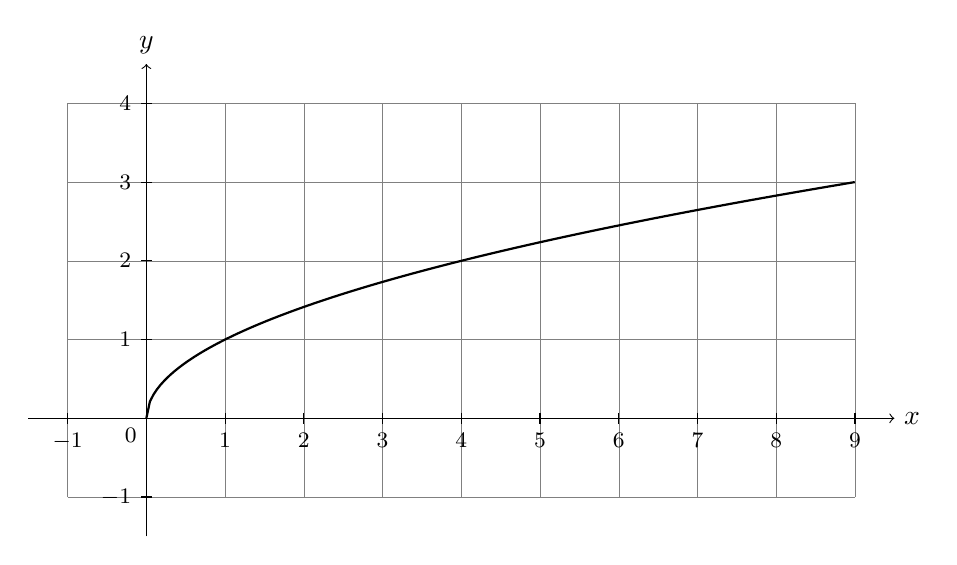
\begin{tikzpicture}[x=1cm,y=1cm]
\draw[help lines] (-1,-1) grid (9,4);
\draw[->] (-1.5,0) -- (9.5,0) node[right] {$x$};
\draw[->] (0,-1.5) -- (0,4.5) node[above] {$y$};
\foreach \x in {-1,1,2,...,9}
	\draw[shift={(\x,0)}] (0pt,2pt) -- (0pt,-2pt) node[below] {\footnotesize $\x$};
\foreach \y in {-1,1,2,...,4}
	\draw[shift={(0,\y)},color=black] (2pt,0pt) -- (-2pt,0pt) node[left] {\footnotesize $\y$};
\draw [domain=0:9,samples=200,thick] plot(\x,{sqrt(\x)});
\node [below left] at (0,0) {\footnotesize 0};
\end{tikzpicture}
%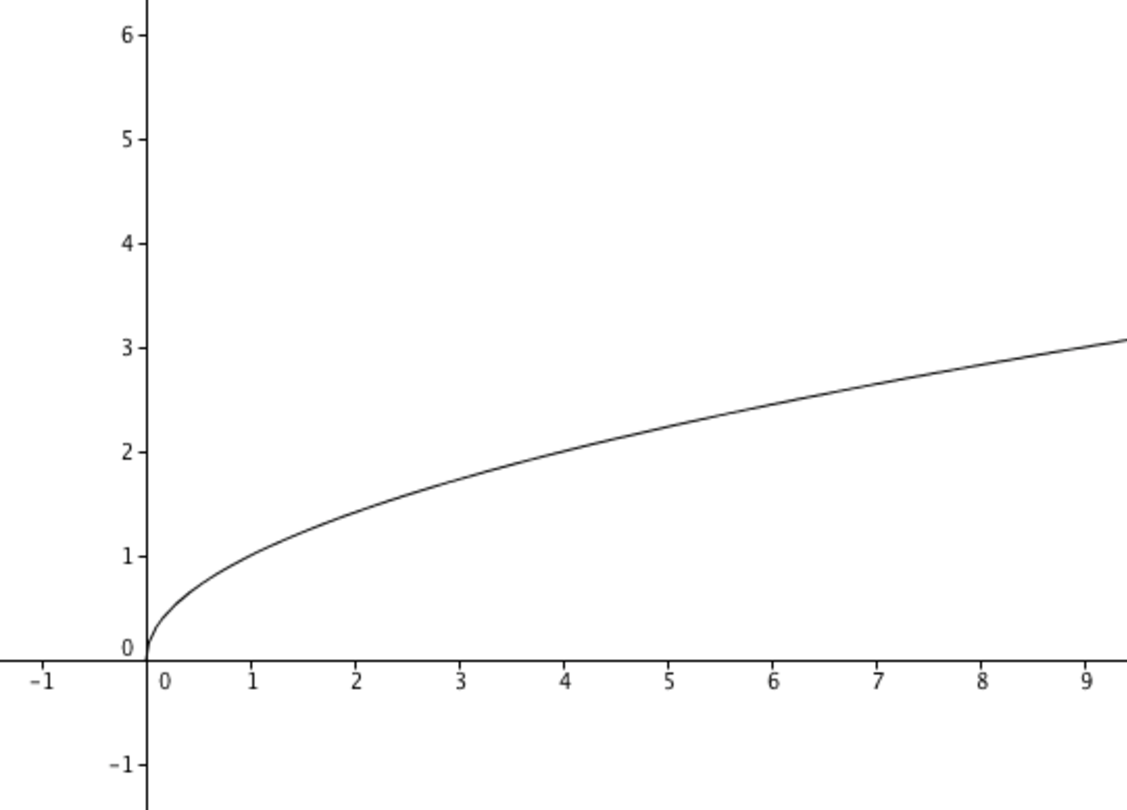
\includegraphics[width=0.5\textwidth]{figuren/verzamelingen_relaties/opl_oef26}
\caption{Oplossing van oefening~\ref{oef:26} }
\label{oef:opl26}
\end{figure}
\end{enumerate}


\item
\begin{enumerate}
\item bron- en beeldverzameling is  $\mathbb{R}^+$
\item $U=\{(x,y)|x,y\in \mathbb{R}^+\text{ en } y=8,48175\cdot x/100\}$
\end{enumerate}
\item
\begin{enumerate}
\item bron- en beeldverzameling is  $\mathbb{R}^+$
\item $U=\left\lbrace(x,y)|x,y\in \mathbb{R}^+\text{ en } y=
\begin{cases}
0,9155\cdot x&\text{ als }x<2000\\
0,8887\cdot x&\text{ anders }
\end{cases} \qquad
\right\rbrace$
\end{enumerate}

\end{enumerate}
\end{Oplossing}
\begin{Oplossing}{2.7}
\item \{(7,1),(10,2),(9,3) \}
\item
\begin{tabular}{c|cccccc}
$y$ & 2 & 4 & 6 & 8 & 10 & 12 \\
\midrule
$x$ & \num{0.1} & \num{0.2} & \num{0.3} & \num{0.4} & \num{0.5} & \num{0.6} \\
\end{tabular}
\item $f^{-1}: \mathbb{R}\rightarrow\mathbb{R}:x\mapsto  y=\dfrac{x-10}{2} $
\item $f^{-1}: \mathbb{R}^+\rightarrow\mathbb{R}^+:x\mapsto y=x^2$
\end{Oplossing}
\begin{Oplossing}{2.8}
\begin{enumerate}
\item $y=-\frac52 x +10$; inverse functie: $y=-\frac25 x +4$
\item $y=2x-5$; inverse functie: $y=\frac12 x+\frac52$
\item $y=-\frac25x-2$; inverse functie: $y=-\frac52x-5$
\end{enumerate}
\end{Oplossing}
\begin{Oplossing}{3.1}
\begin{enumerate}
\item $f(x)=-3x+11$, nulpunt $(\frac{11}{3}, 0)$ en snijpunt met de $y$-as: $(0,11)$
\item $f(x)=-4$, dus een constante functie. Deze functie heeft geen nulpunt en het snijpunt met de $y$-as is $(0,-4)$.
\item Deze rechte heeft als vergelijking $x=3$. Het is een verticale rechte en dus geen functie. Het heeft dan ook geen zin om te spreken over nulpunt en snijpunt met de $y$-as.
\end{enumerate}
     
\end{Oplossing}
\begin{Oplossing}{3.2}
 Enkel rechte $d$ is geen functie \\
$a\leftrightarrow y=-\frac{1}{2}x$\\
$b \leftrightarrow y=-4 $\\
$c \leftrightarrow y=x+3$\\
$d \leftrightarrow x=3$
\end{Oplossing}
\begin{Oplossing}{3.3}
Tot een maandelijkse beltijd van 37,5 minuten is Base het goedkoopst. Tussen 37,5 en 120 minuten kan je best Mobistarklant worden. Voor wie meer belt dan twee uur per maand is Proximus het goedkoopst.
Voor 10 belminuten kies je dus Base met een kostprijs van $10\cdot 0,40=4$ euro. Als je 100 minuten per maand belt, ben je goedkoopst bij Mobistar. Dat kost je dan \euros{25}. Wie 1000 minuten belt, hoeft niet te twijfelen: kies Proximus en dus kost het je \euros{30}.
\end{Oplossing}
\begin{Oplossing}{3.4}
Eerst en vooral: de aanname van rechtevenredigheid is niet te verdedigen. Als je naar de geciteerde URL in de opgave gaat kijken, merk je dat men niet anders kan dan ook het verbruik (koeling, \ldots) in aanmerking nemen en proberen dit zo laag mogelijk te houden. Als we dan toch de evenredigheid volgen, bekomen we het antwoord dat getoond wordt in figuur~\ref{fig:rekensnelheidvermogen}.
\begin{figure}[htbp]
    \centering
\begin{tikzpicture}[x=0.08cm,y=0.15cm]
%\draw[help lines] (-5,-5) grid  (5,5);
\draw[->] (-2,0) -- (105,0) node[right] {1000 TFlops};
\draw[->] (0,-1) -- (0,52) node[above] {\si{\mega\watt}};
\foreach \x in {10,20,...,100}
	\draw[shift={(\x,0)}] (0pt,2pt) -- (0pt,-2pt) node[below] {\footnotesize $\x$};
\foreach \y in {10,20,...,50}
	\draw[shift={(0,\y)},color=black] (2pt,0pt) -- (-2pt,0pt) node[left] {\footnotesize $\y$};
\node [below left] at (0,0) {\footnotesize 0};
\draw[thick] (0,0) -- (110,53.17);
\draw[dashed] (16.324,0) |- (0,7.89);
\filldraw [red] (16.324,7.89) circle (2pt) node[below right] {$(16,324;7,89)$};
\draw[dashed] (100,0) |- (0,48.33);
\filldraw [red] (100,48.33) circle (2pt) node[below right] {$(100;48,33)$};
\end{tikzpicture}
\caption{Verband tussen vermogen en rekensnelheid}
    \label{fig:rekensnelheidvermogen}
\end{figure}
\end{Oplossing}
\begin{Oplossing}{3.5}
Stel de vergelijking van de rechte door de punten $(500,60)$ en $(2000,130)$. Vul dan in deze vergelijking $x=1500$ in en je bekomt \euros{106,67}. Bij 5 TB spreken we over extrapolatie en dat is meestal vrij gevaarlijk. Hoe meer data op een harde schijf, des te groter wordt de technische uitdaging en des te kleiner worden componenten, sporen enz. Een lineair verband zal dan zeker geen goede benadering zijn!
\end{Oplossing}
\begin{Oplossing}{3.6}
\begin{enumerate}
\item Veranderlijken benoemen: $x$ is verbruikte hoeveelheid drinkwater; $B$ is het te betalen bedrag
\item $B(x)=47+(2+0,9+1,3)\cdot x=47+4,2x$
\item $B_2(x)=47+2\cdot (x-15)+(0,9+1,3)\cdot x=17+4,2\cdot x$ \\
$B_2(45)=206$. De gemiddelde Vlaming betaalt \euros{206} per jaar.
\end{enumerate}
\end{Oplossing}
\begin{Oplossing}{3.7}
$\qquad$ \\
\begin{lstlisting}[caption={Drinkwaterverbruik in Vlaanderen en in Brussel}]
function y=vlaanderen(x)
    if x<0 then
        error("verbruik moet positief zijn")
    end
    if x<15 then
        y=2.2*x
    else
        y=2.2*x+2*(x-15)
    end
endfunction

function y=brussel(x)
    if x<0 then
        error("verbruik moet positief zijn")
    end
    if x<15 then
        y=1.88*x
    elseif x<30
        y=1.88*15+3.38*(x-15)
    elseif x<60
        y=1.88*15+3.38*15+4*(x-30)
    else
        y=1.88*15+3.38*15+4*30+7.33*(x-60)
    end
endfunction

clf
x=0:80
xgrid
plot(x,vlaanderen)
plot(x,brussel,"r")

function y=drinkwater(x,regio)
    if regio<>"vlaanderen"&regio<>"brussel" then
        error("je geeft geen geldige regio")
    end
    if regio=="vlaanderen" then
        y=vlaanderen(x)
    else
        y=brussel(x)
    end
endfunction

function [prijs,regio]=goedkoopste(x)
    if x<0 then
        error("verbruik moet positief zijn")
    end
    vlndr=vlaanderen(x)
    brsl=brussel(x)
    if vlndr<brsl then
        prijs=vlndr
        regio="vlaanderen"
    else
        prijs=brsl
        regio="brussel"
    end
endfunction


[p,r]=goedkoopste(20)
printf("Bij verbruik van 20 eenheden is regio %s het goedkoopst.\n
		De prijs bedraag %f.",r,p)
\end{lstlisting}
\end{Oplossing}
\begin{Oplossing}{3.8}
$\qquad$ \\
\begin{lstlisting}[caption={Likes - controle}]
function y=like(x)
    if x<0 then
        error("het aantal likes moet positief zijn")
    end
    if x<=1000 then
        y=x
    elseif x<=5000
        y=1000+0.80*(x-1000)
    else
        y=1000+0.80*4000+1.20*(x-5000)
    end
endfunction

clf
x=0:7000
xgrid
plot(x,like)

like(4320)
\end{lstlisting}

Bij 4320 likes stort het bedrijf \euros 3656.
\end{Oplossing}
\begin{Oplossing}{4.1}
     De goedkoopste oplossing (figuur~\ref{fig:oplrijstsoja}) die aan alle beperkingen voldoet is drie kopjes rijst en twee kopjes sojascheuten, met een kostprijs van \euros{1,40}.
     \begin{figure}[hbtp]
\centering
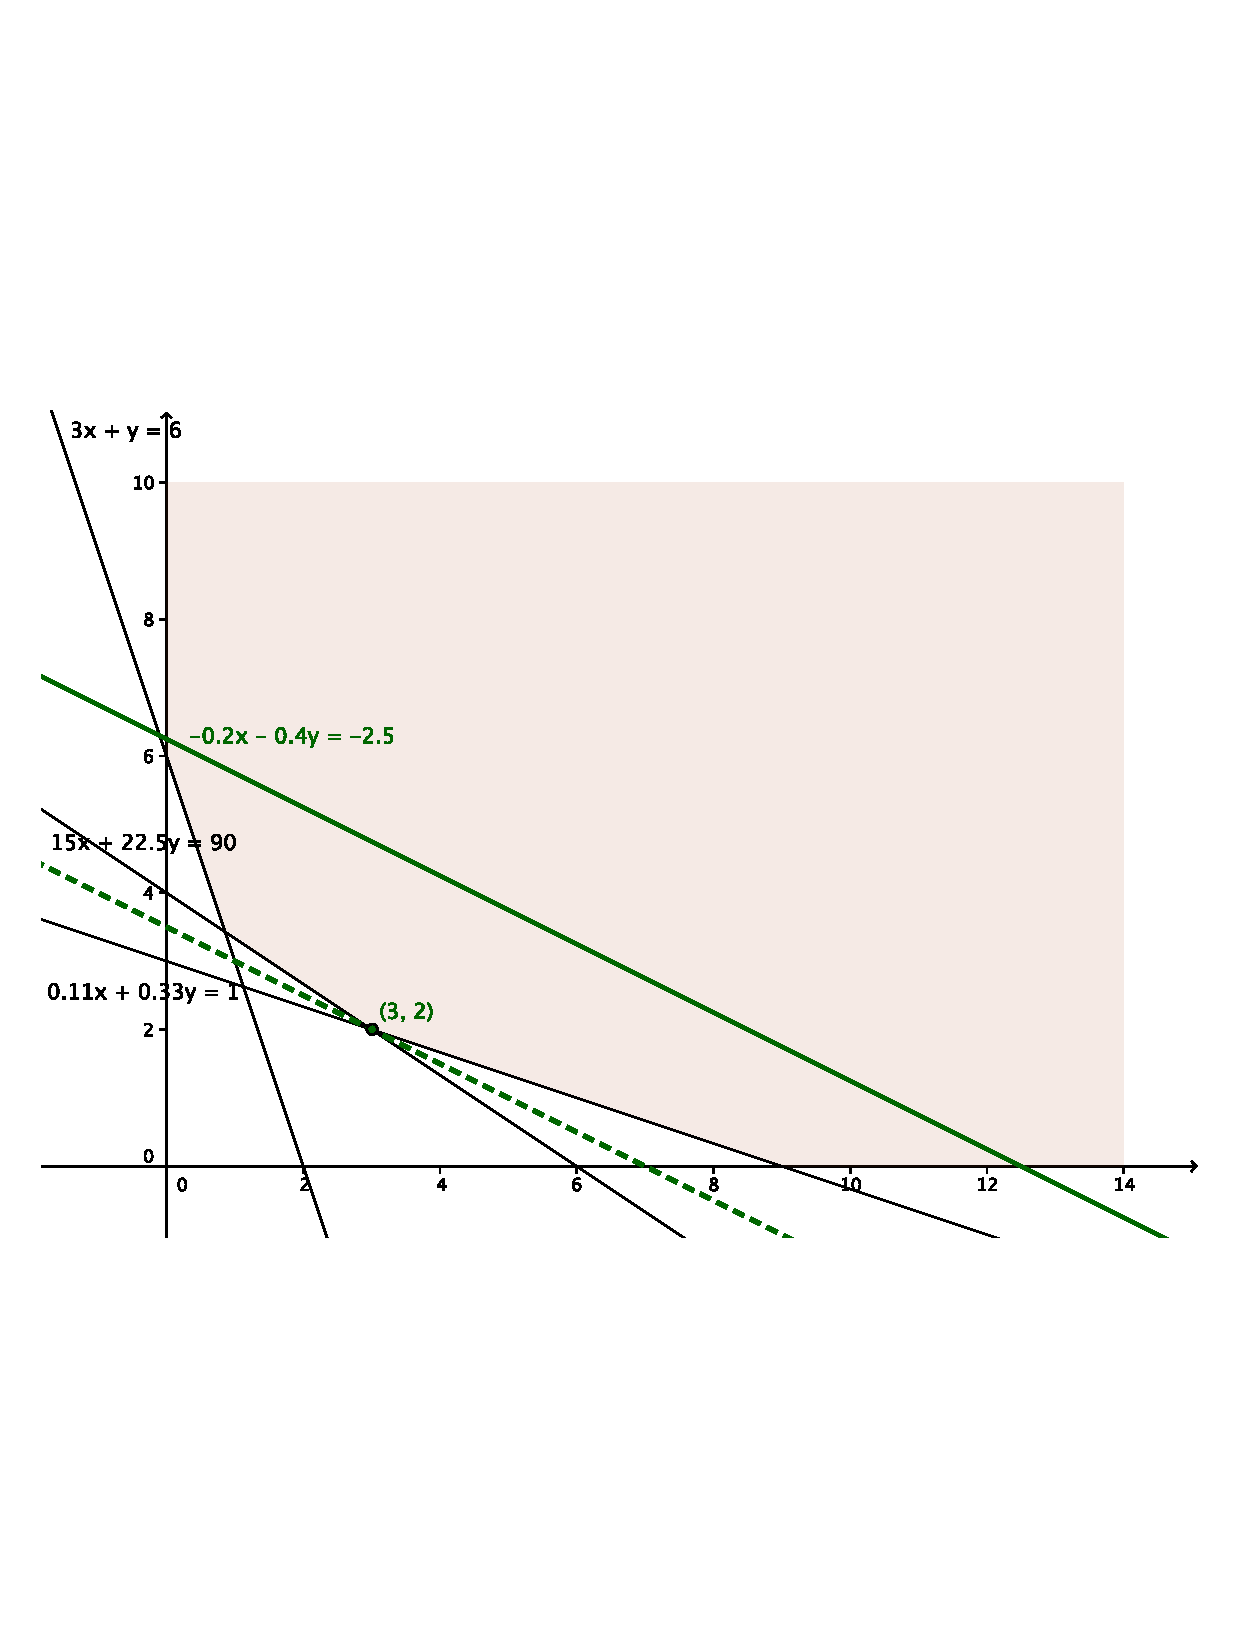
\includegraphics[width=0.8\textwidth]{oefeningen/FigurenLP/OefRijstSoja.pdf}
\caption{Optimaal punt is drie kopjes rijst en twee kopjes soja}
\label{fig:oplrijstsoja}
\end{figure}

     
\end{Oplossing}
\begin{Oplossing}{4.2}
     Vier kasten van type A en acht kasten van type  B leveren de goedkoopste prijs van \euros{3000} en voldoen aan alle voorwaarden (figuur~\ref{fig:kastenAB}).
          \begin{figure}[hbtp]
\centering
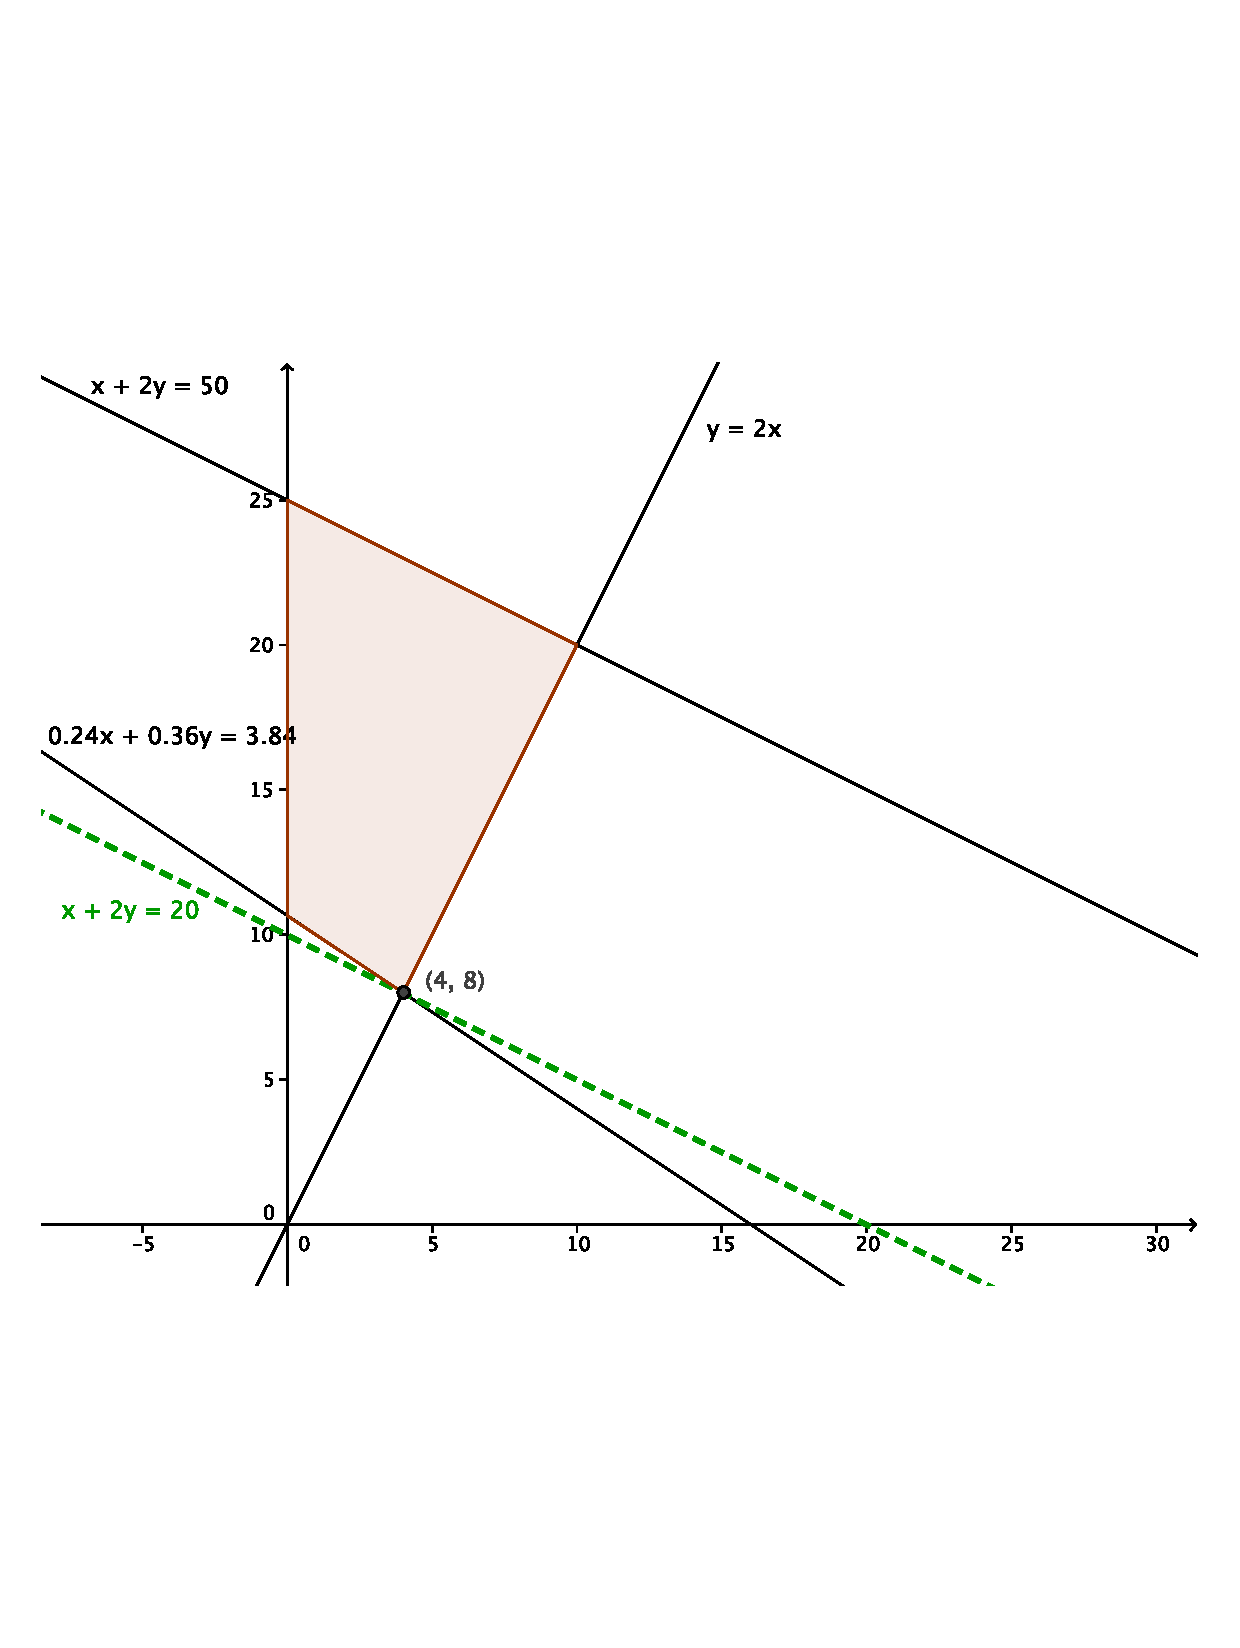
\includegraphics[width=0.8\textwidth]{oefeningen/FigurenLP/OefkastenAB.pdf}
\caption{Optimaal punt is vier kasten A en acht kasten B}
\label{fig:kastenAB}
\end{figure}
     
\end{Oplossing}
\begin{Oplossing}{4.3}
    Tien Fokkers en vijf Boeings leveren de goedkoopste transportoplossing (figuur~\ref{fig:deptjaar}) met een kostprijs van \euros{700\,000}.
              \begin{figure}[hbtp]
\centering
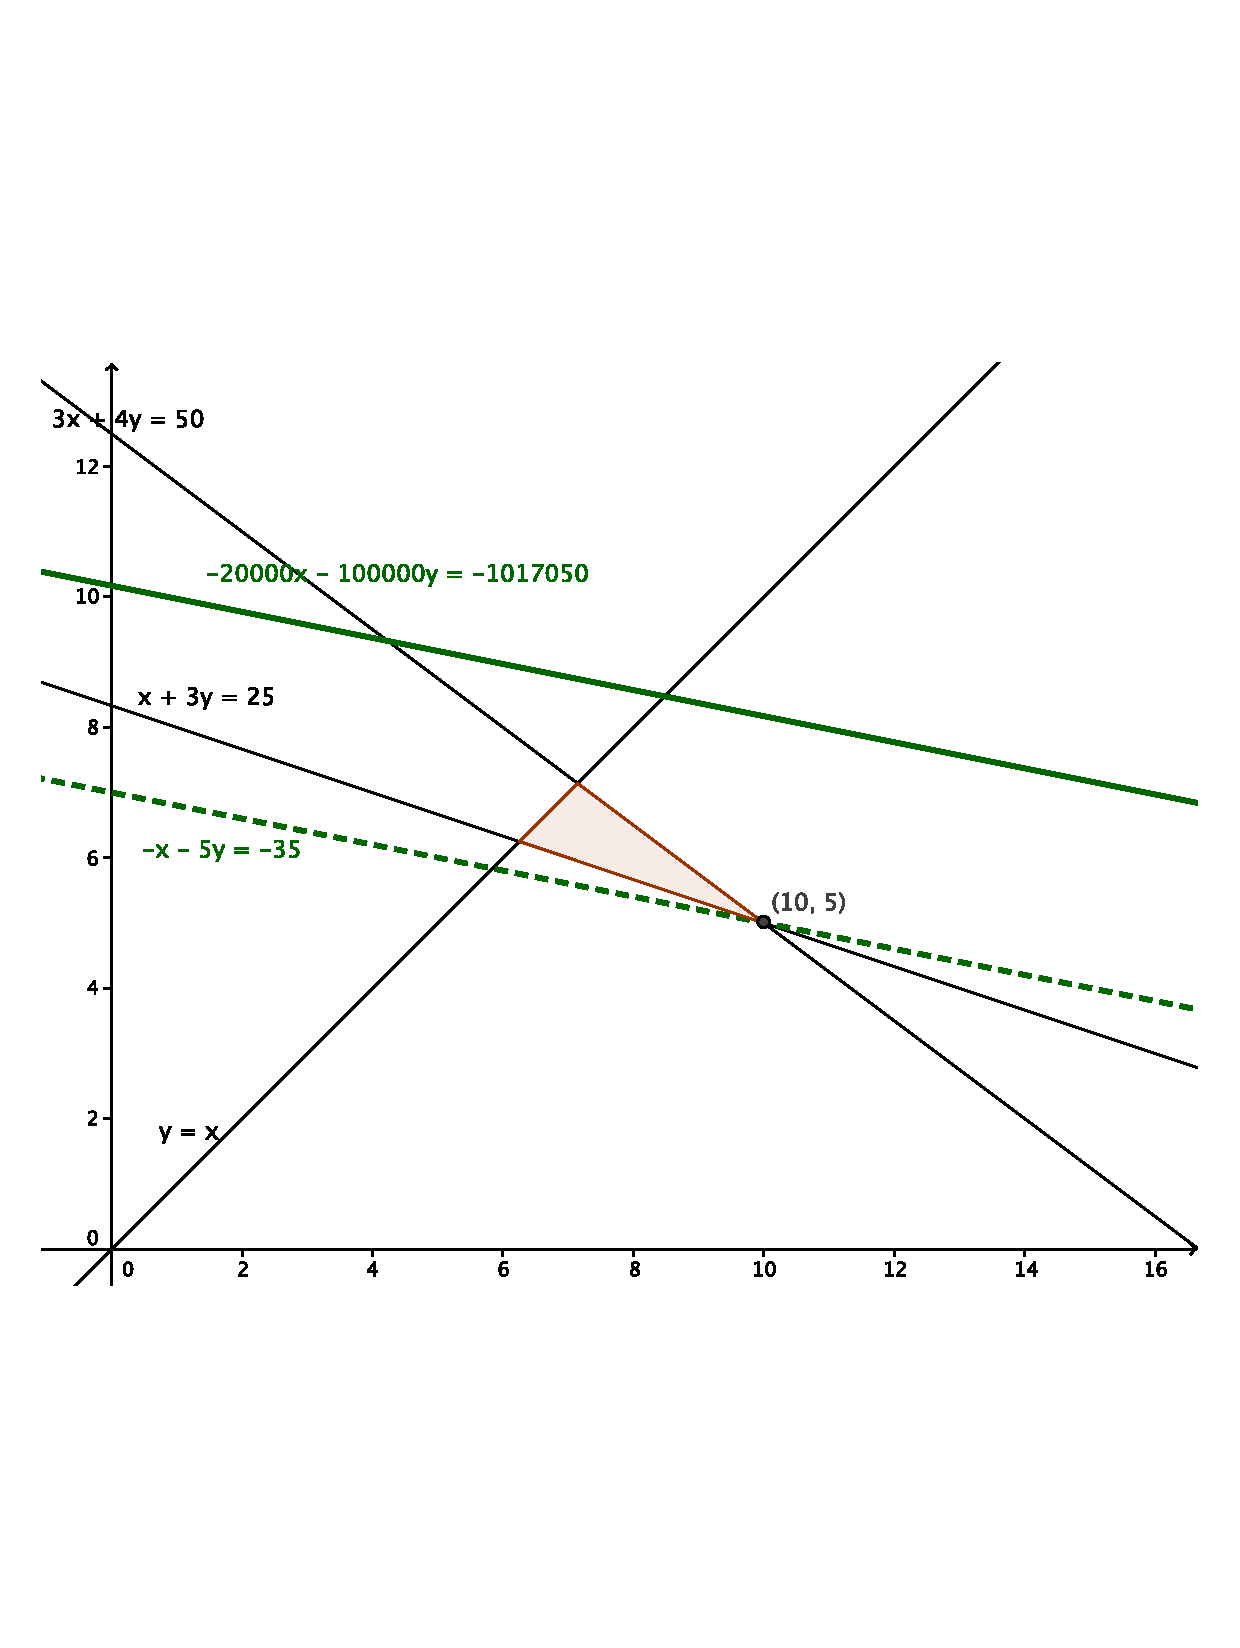
\includegraphics[width=0.8\textwidth]{oefeningen/FigurenLP/OefDepvhjaar.pdf}
\caption{Optimaal punt is 10 Fokkers en 5 Boeings}
\label{fig:deptjaar}
\end{figure}
    \clearpage
    
\end{Oplossing}
\begin{Oplossing}{4.4}
     Met 2000 tenten en 6000 dekens kunnen in totaal 16\,000 mensen geholpen worden (figuur~\ref{fig:AZG}).
                   \begin{figure}[hbtp]
\centering
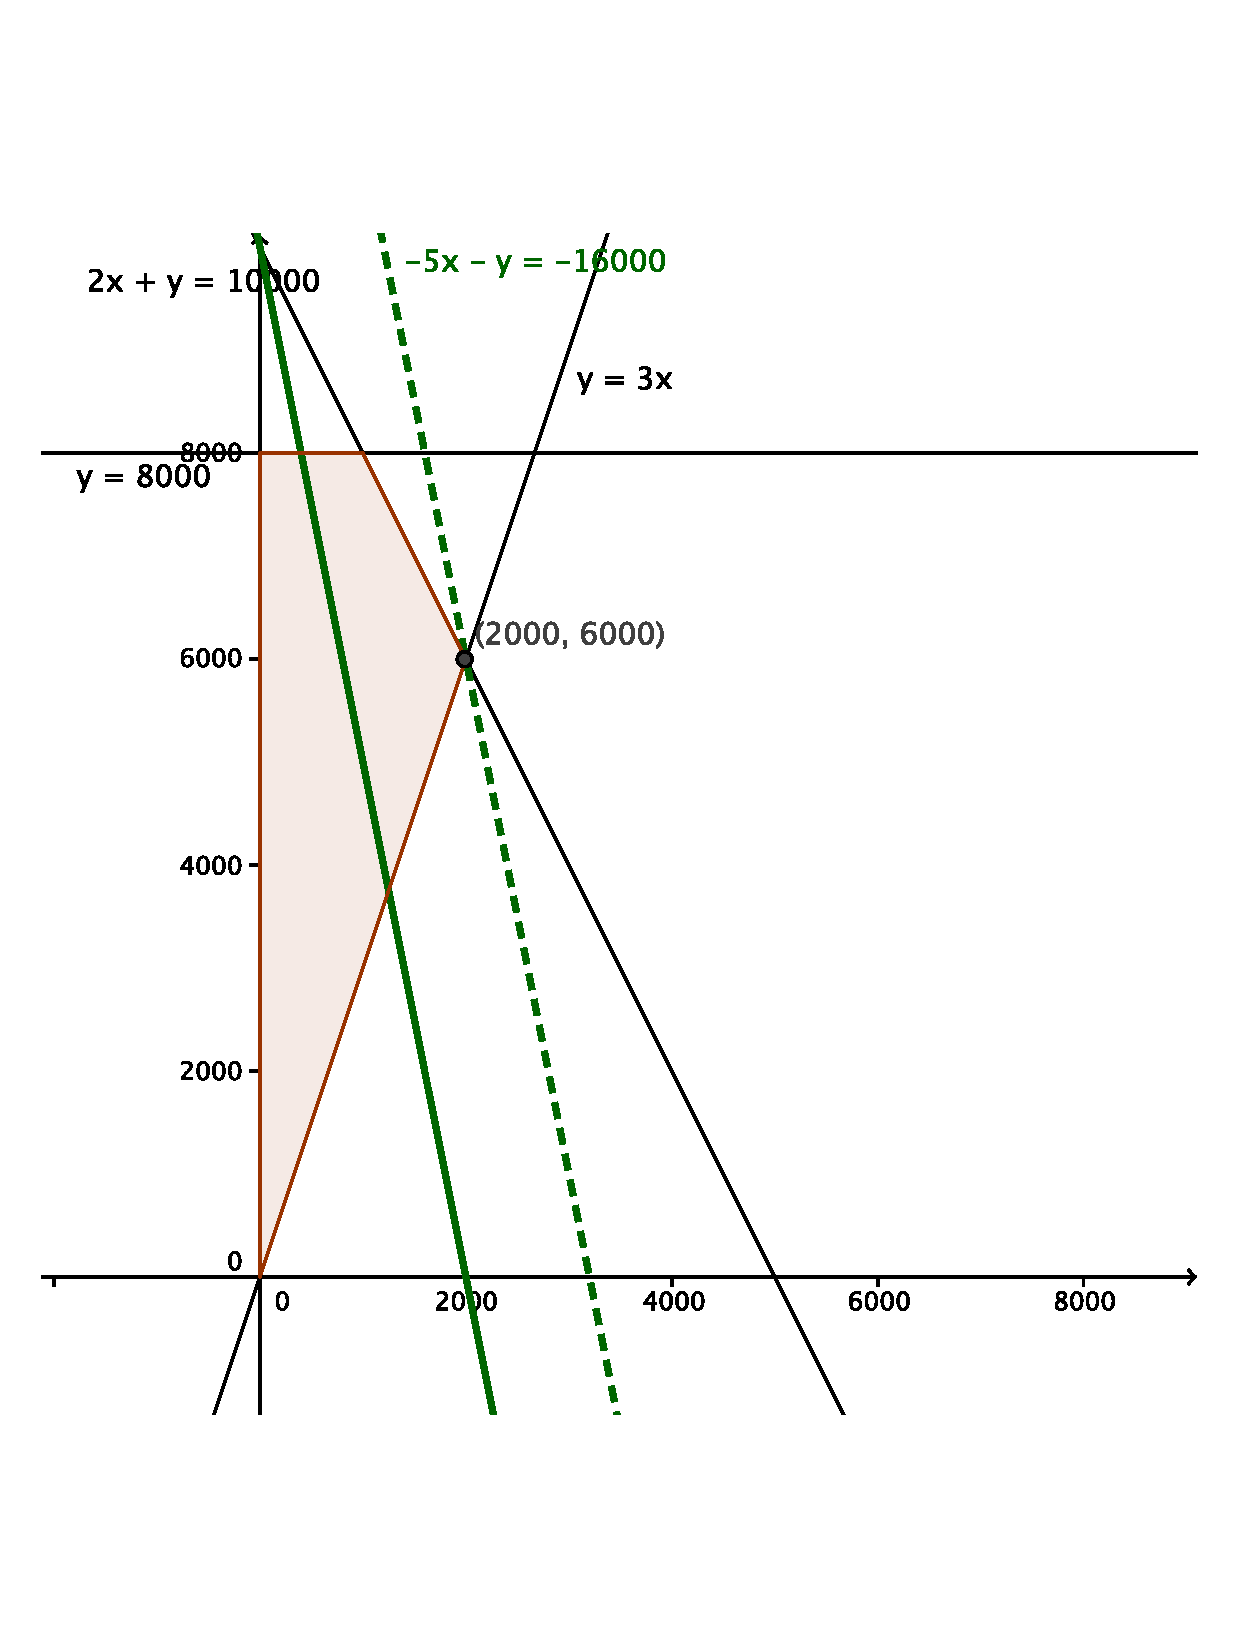
\includegraphics[width=0.7\textwidth]{oefeningen/FigurenLP/OefAZG.pdf}
\caption{Optimaal punt is 2000 tenten en 6000 dekens}
\label{fig:AZG}
\end{figure}
     
\end{Oplossing}
\begin{Oplossing}{4.6}
     20 ha ma\"is, 18 ha aardappelen
     
\end{Oplossing}
\begin{Oplossing}{4.7}
        10 tafels en 15 stoelen (figuur~\ref{fig:tafelstoelen}) leveren de grootste winst, nl \euros{2375}.
        \begin{figure}[hbtp]
\centering
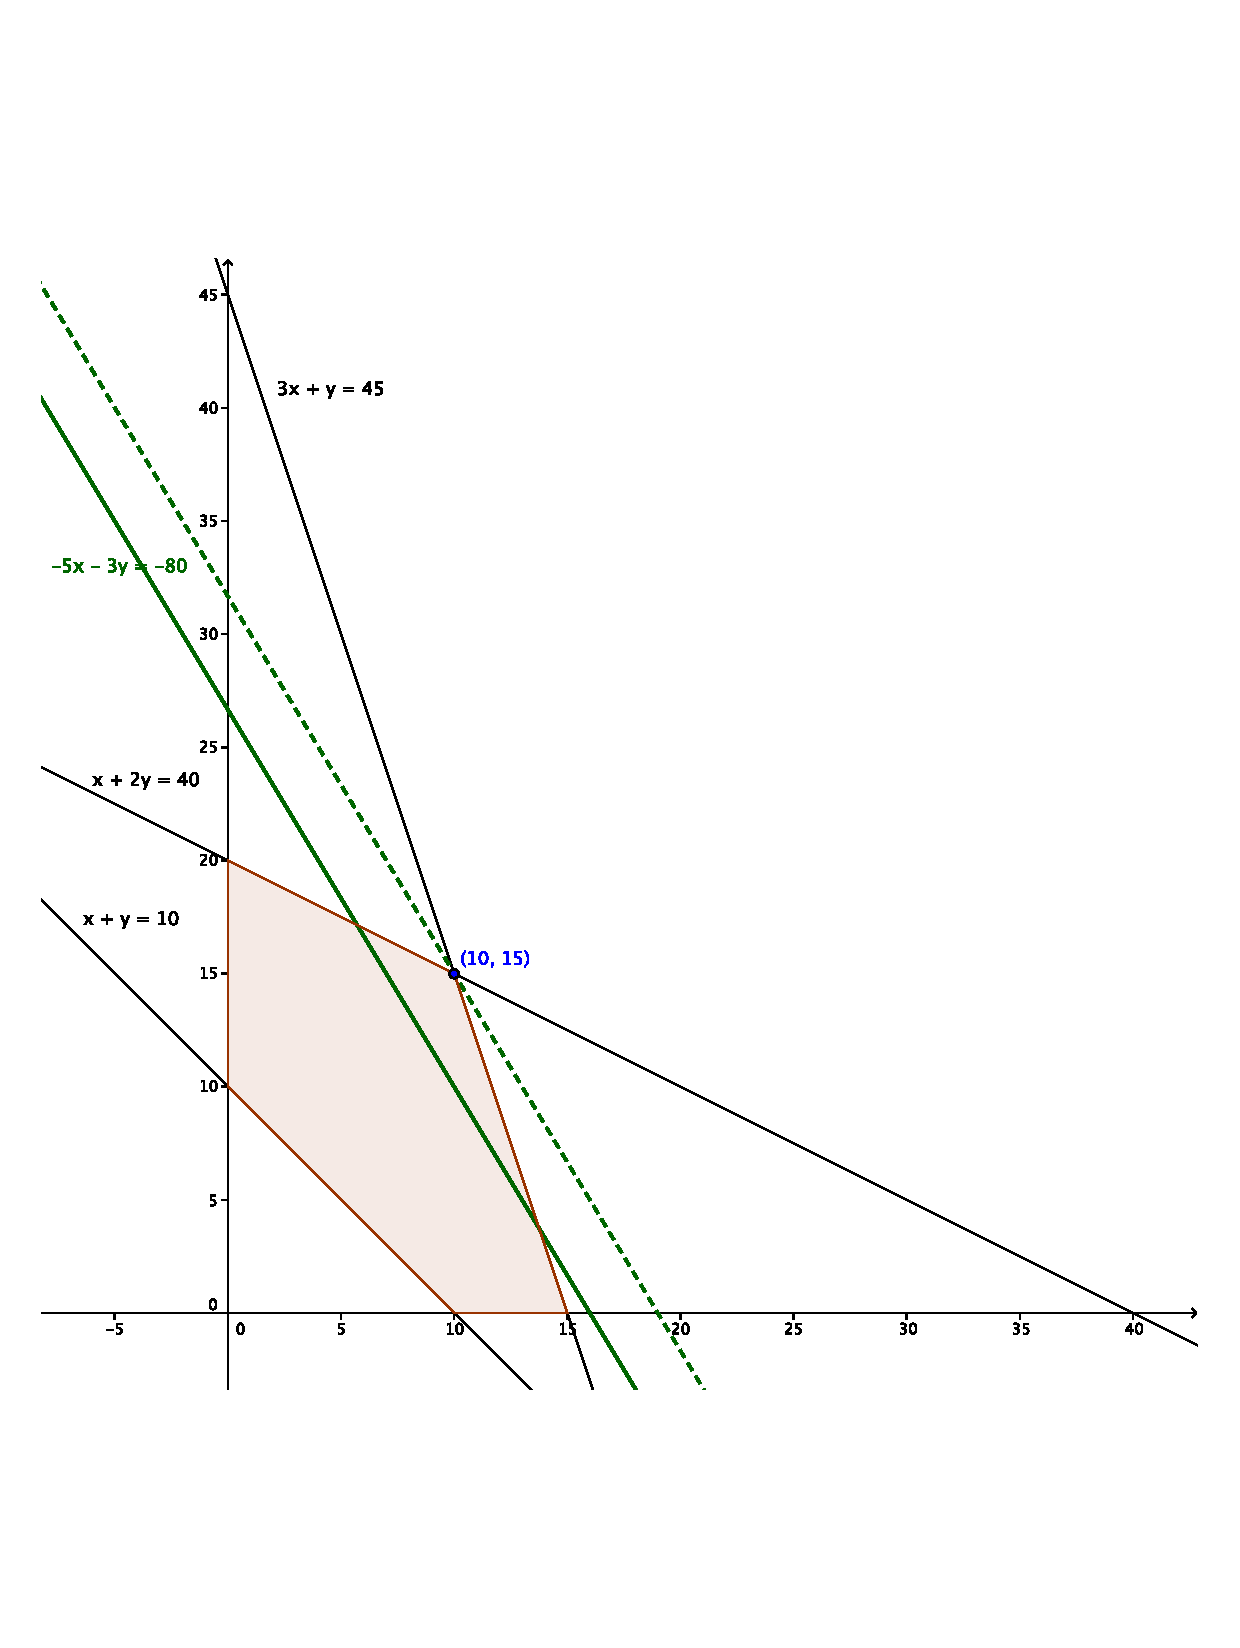
\includegraphics[width=0.8\textwidth]{oefeningen/FigurenLP/Oef7.pdf}
\caption{10 tafels en 15 stoelen leveren de grootste winst}
\label{fig:tafelstoelen}
\end{figure}
\clearpage
        
\end{Oplossing}
\begin{Oplossing}{4.8}
    De maximale winst (\euros{102\,000}) wordt bereikt bij de productie van 36 containers van type A en 12 containers van type B (figuur~\ref{fig:containersAB}).
            \begin{figure}[hbtp]
\centering
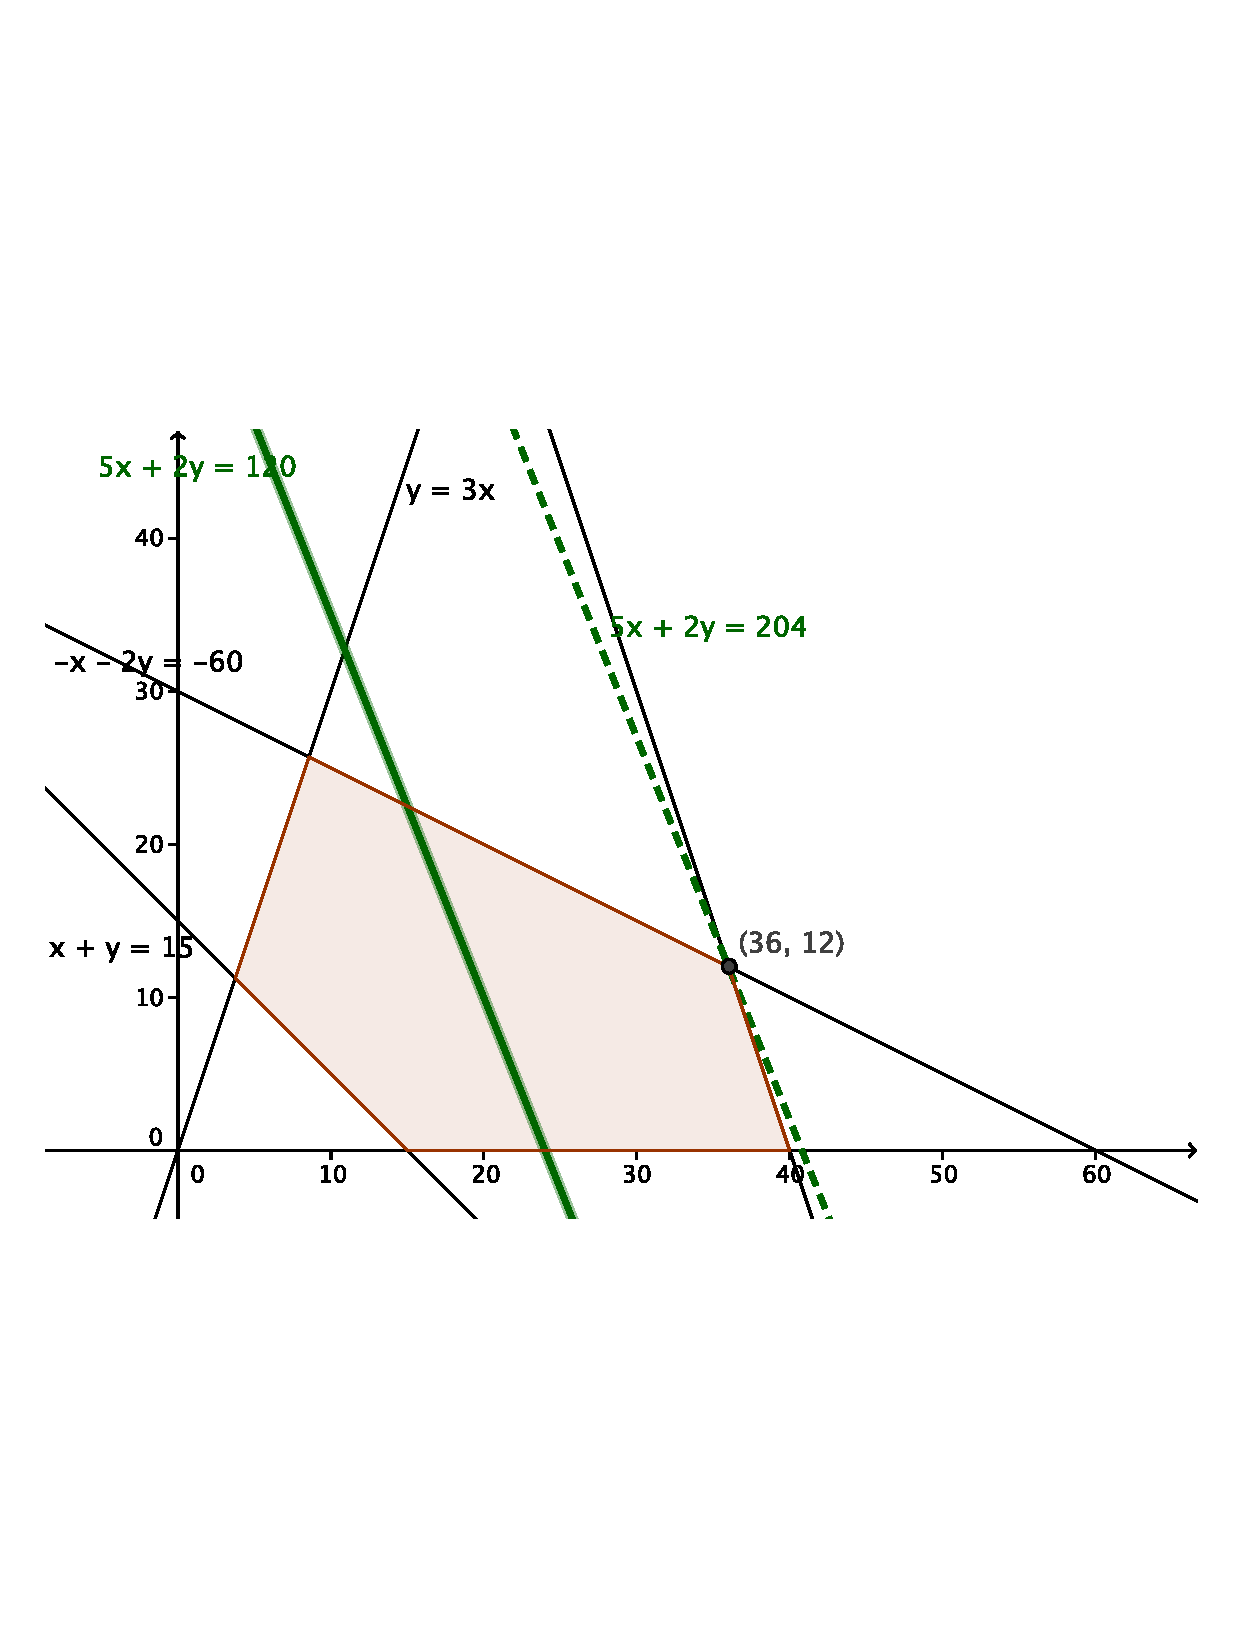
\includegraphics[width=0.8\textwidth]{oefeningen/FigurenLP/OefcontainersAB.pdf}
\caption{De grootste winst is bij 36 containers A en 12 containers B}
\label{fig:containersAB}
\end{figure}
    
\end{Oplossing}
\begin{Oplossing}{4.9}
     Een maandproductie van 20 ton platen en 30 ton buizen (figuur~\ref{fig:platenbuizen}) levert de maximale winst van \euros{110\,000}.
                 \begin{figure}[hbtp]
\centering
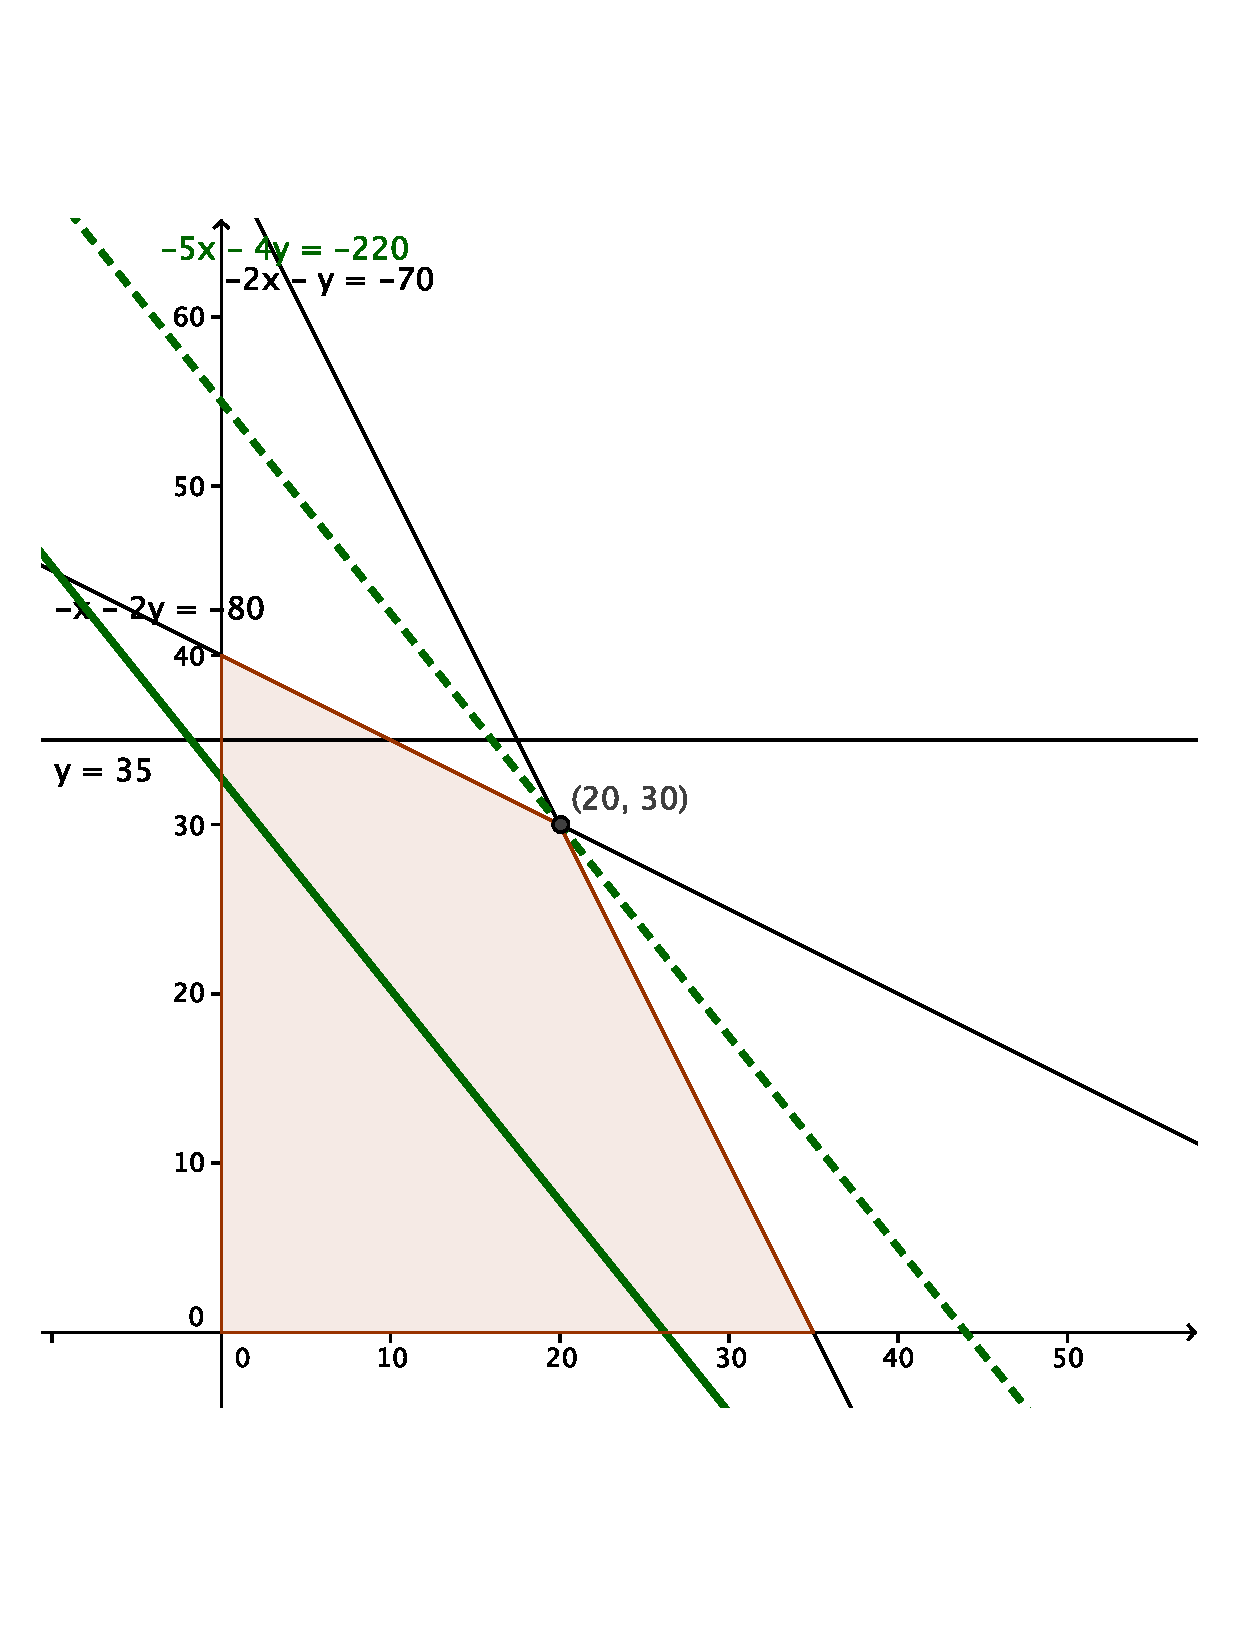
\includegraphics[width=0.8\textwidth]{oefeningen/FigurenLP/OefPlatenBuizen.pdf}
\caption{Maximale winst bij 20 ton platen en 30 ton buizen}
\label{fig:platenbuizen}
\end{figure}
\clearpage
     
\end{Oplossing}
\begin{Oplossing}{4.10}
     15 voorstellingen van elke film
     
\end{Oplossing}
\begin{Oplossing}{4.11}
Als de parking dagelijks 45 auto's en 10 bussen ontvangt (figuur~\ref{fig:autobussen}), is de opbrengst maximaal (\euros{330}).
                 \begin{figure}[hbtp]
\centering
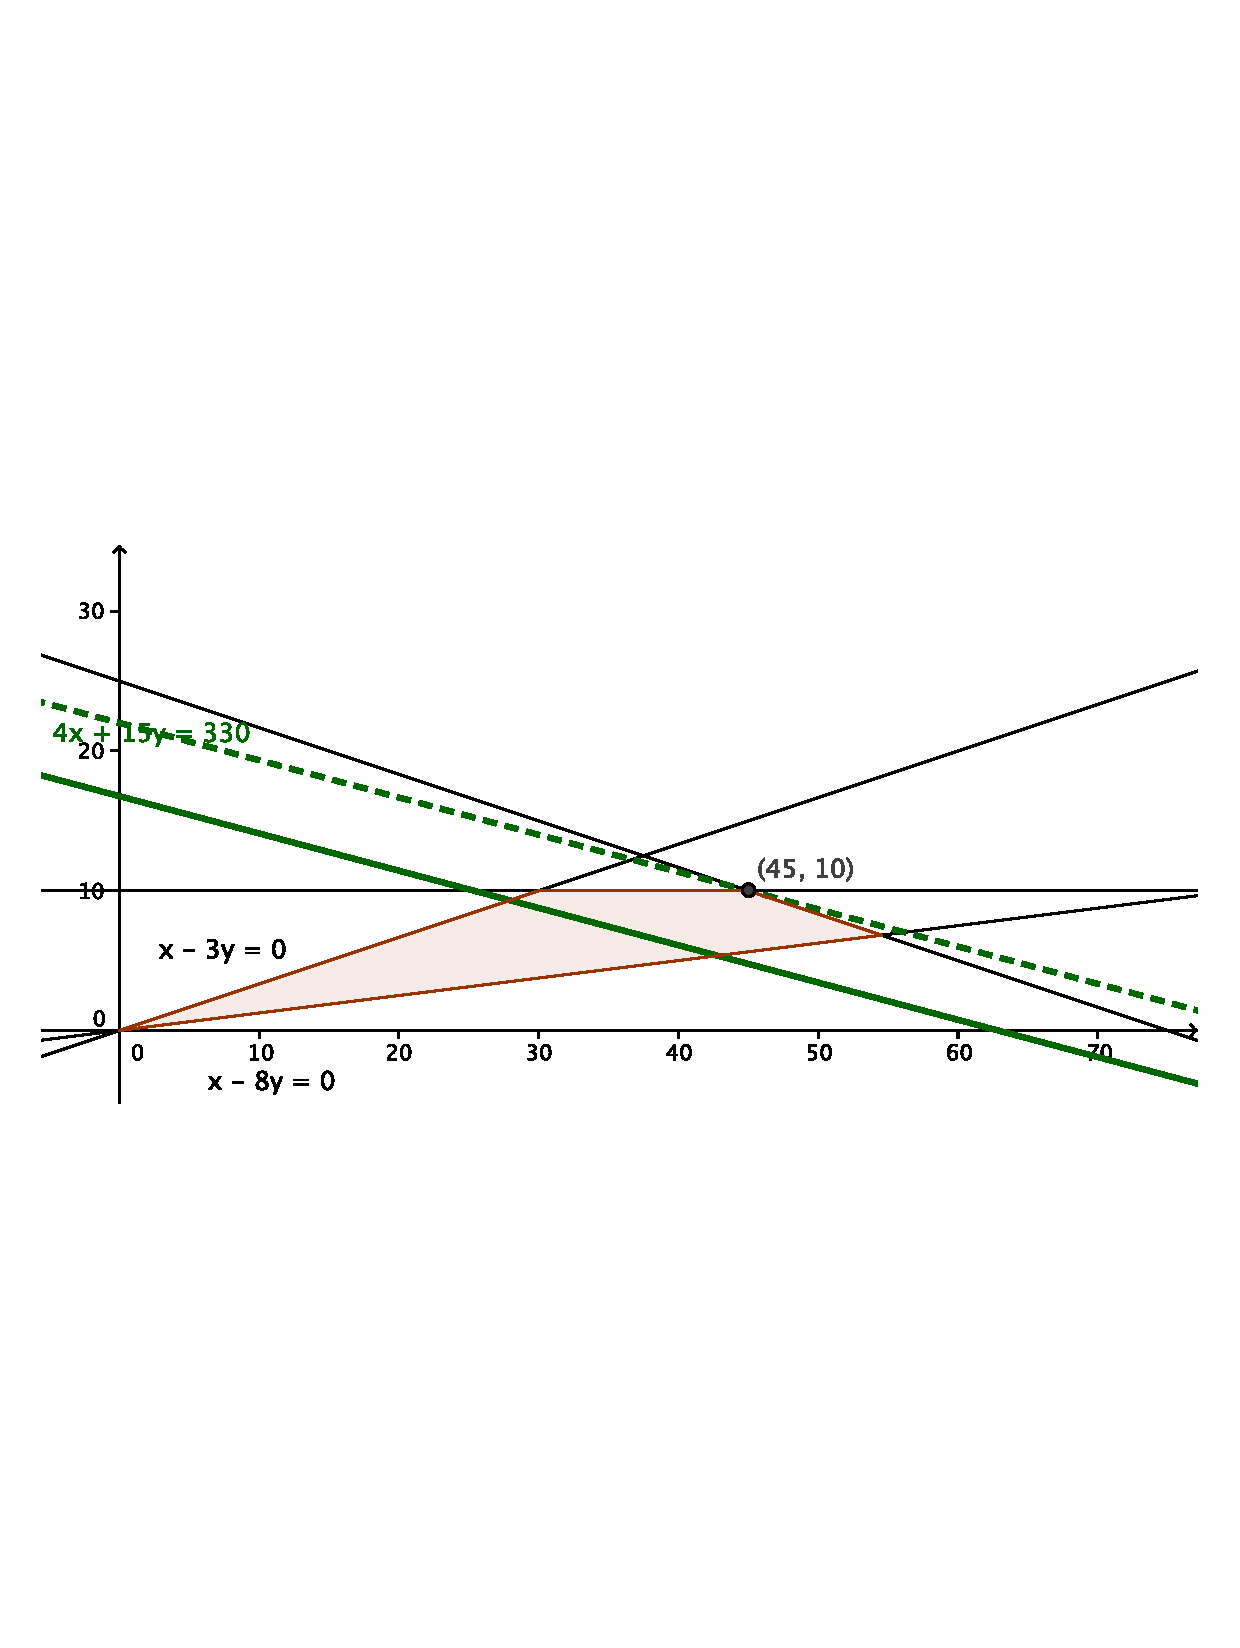
\includegraphics[width=0.8\textwidth]{oefeningen/FigurenLP/Oefautosbussen.pdf}
\caption{Maximale parkingopbrengst bij 45 auto's en 10 bussen}
\label{fig:autobussen}
\end{figure}
\end{Oplossing}
\begin{Oplossing}{4.12}
Als Anne 30 potjes vanille- en 10 potjes chocoladepudding maakt en verkoopt (figuur~\ref{fig:pudding}) heeft ze een maximale opbrengst van \euros{38}.
\begin{figure}[hbtp]
\centering
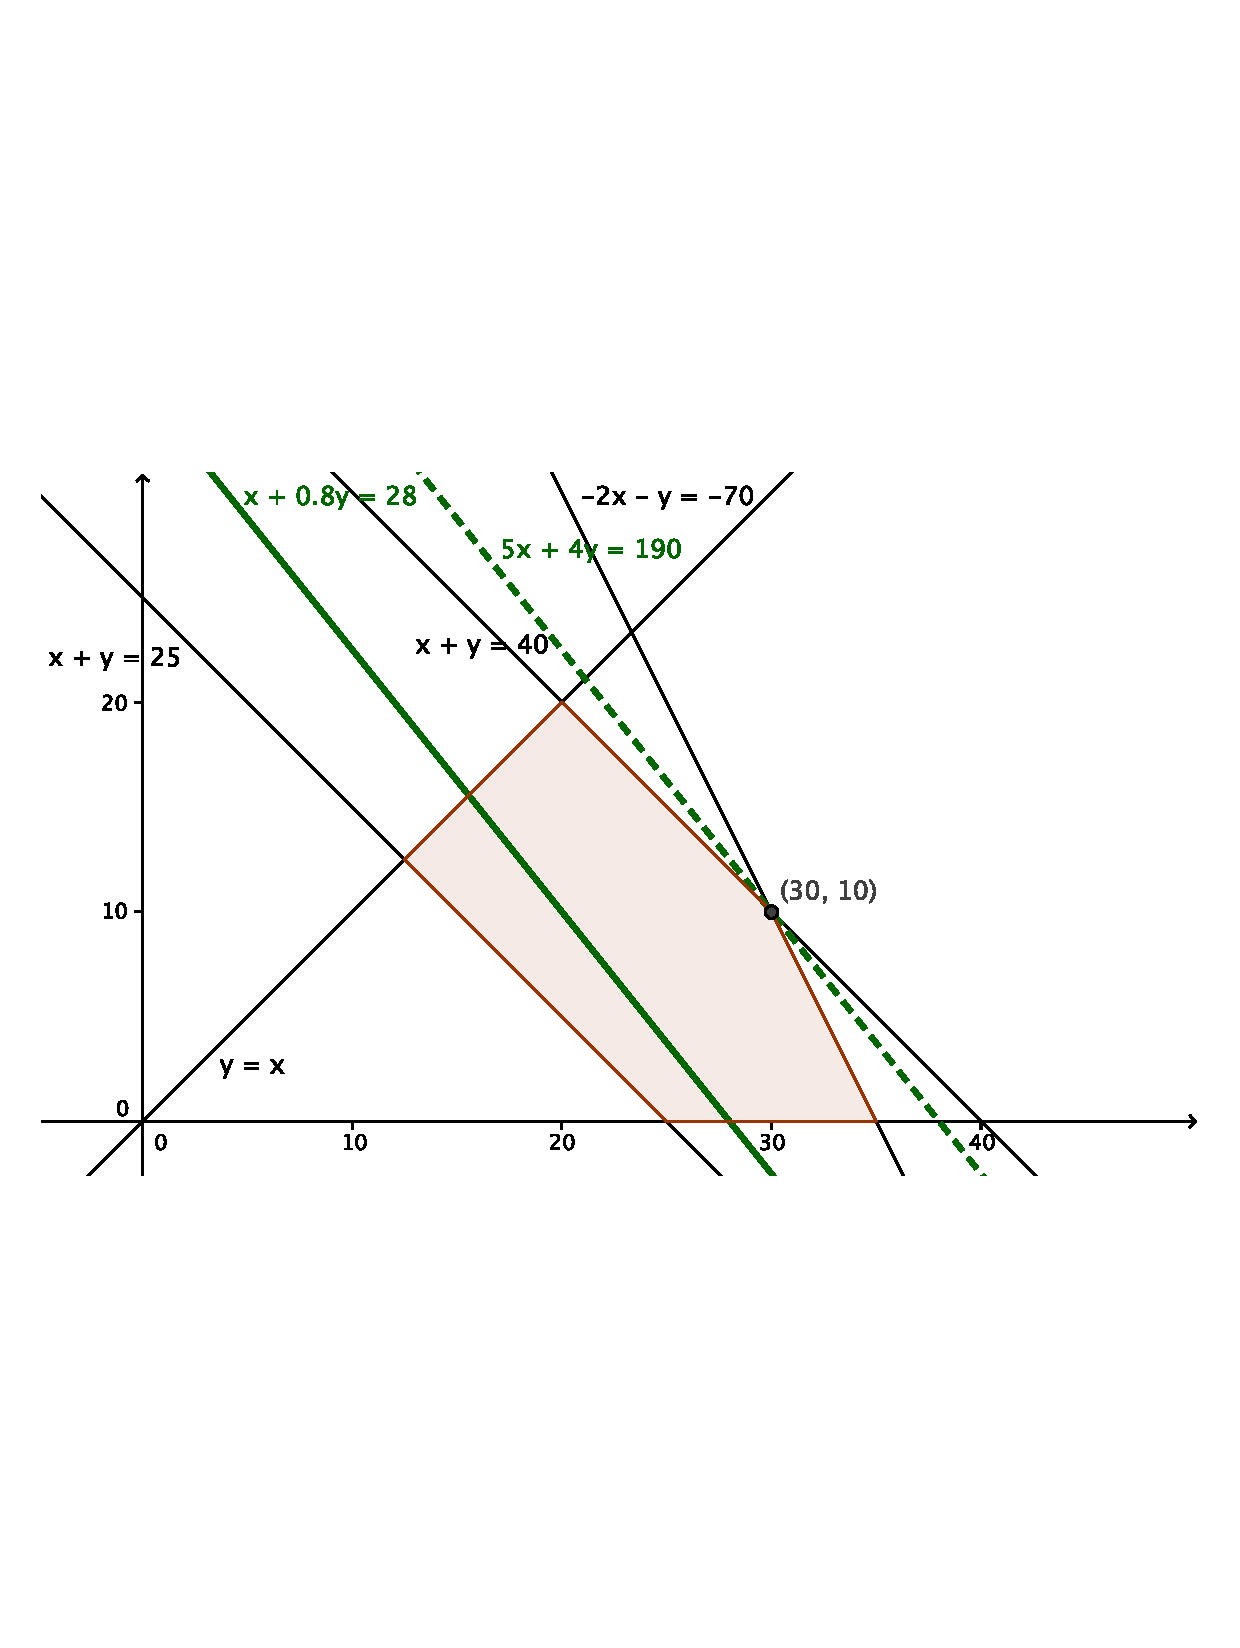
\includegraphics[width=0.8\textwidth]{oefeningen/FigurenLP/Oefpudding.pdf}
\caption{Maximale winst bij 30 potjes vanille- en 10 chocoladepudding}
\label{fig:pudding}
\end{figure}
\end{Oplossing}
\begin{Oplossing}{4.13}
15 vogelkers, 30 eiken
\end{Oplossing}
\begin{Oplossing}{4.14}
50 lofts en 22 appartementen (eigenlijk 22,5 appartementen, maar je kan geen half appartement bouwen)
\begin{figure}[htb]
\centering
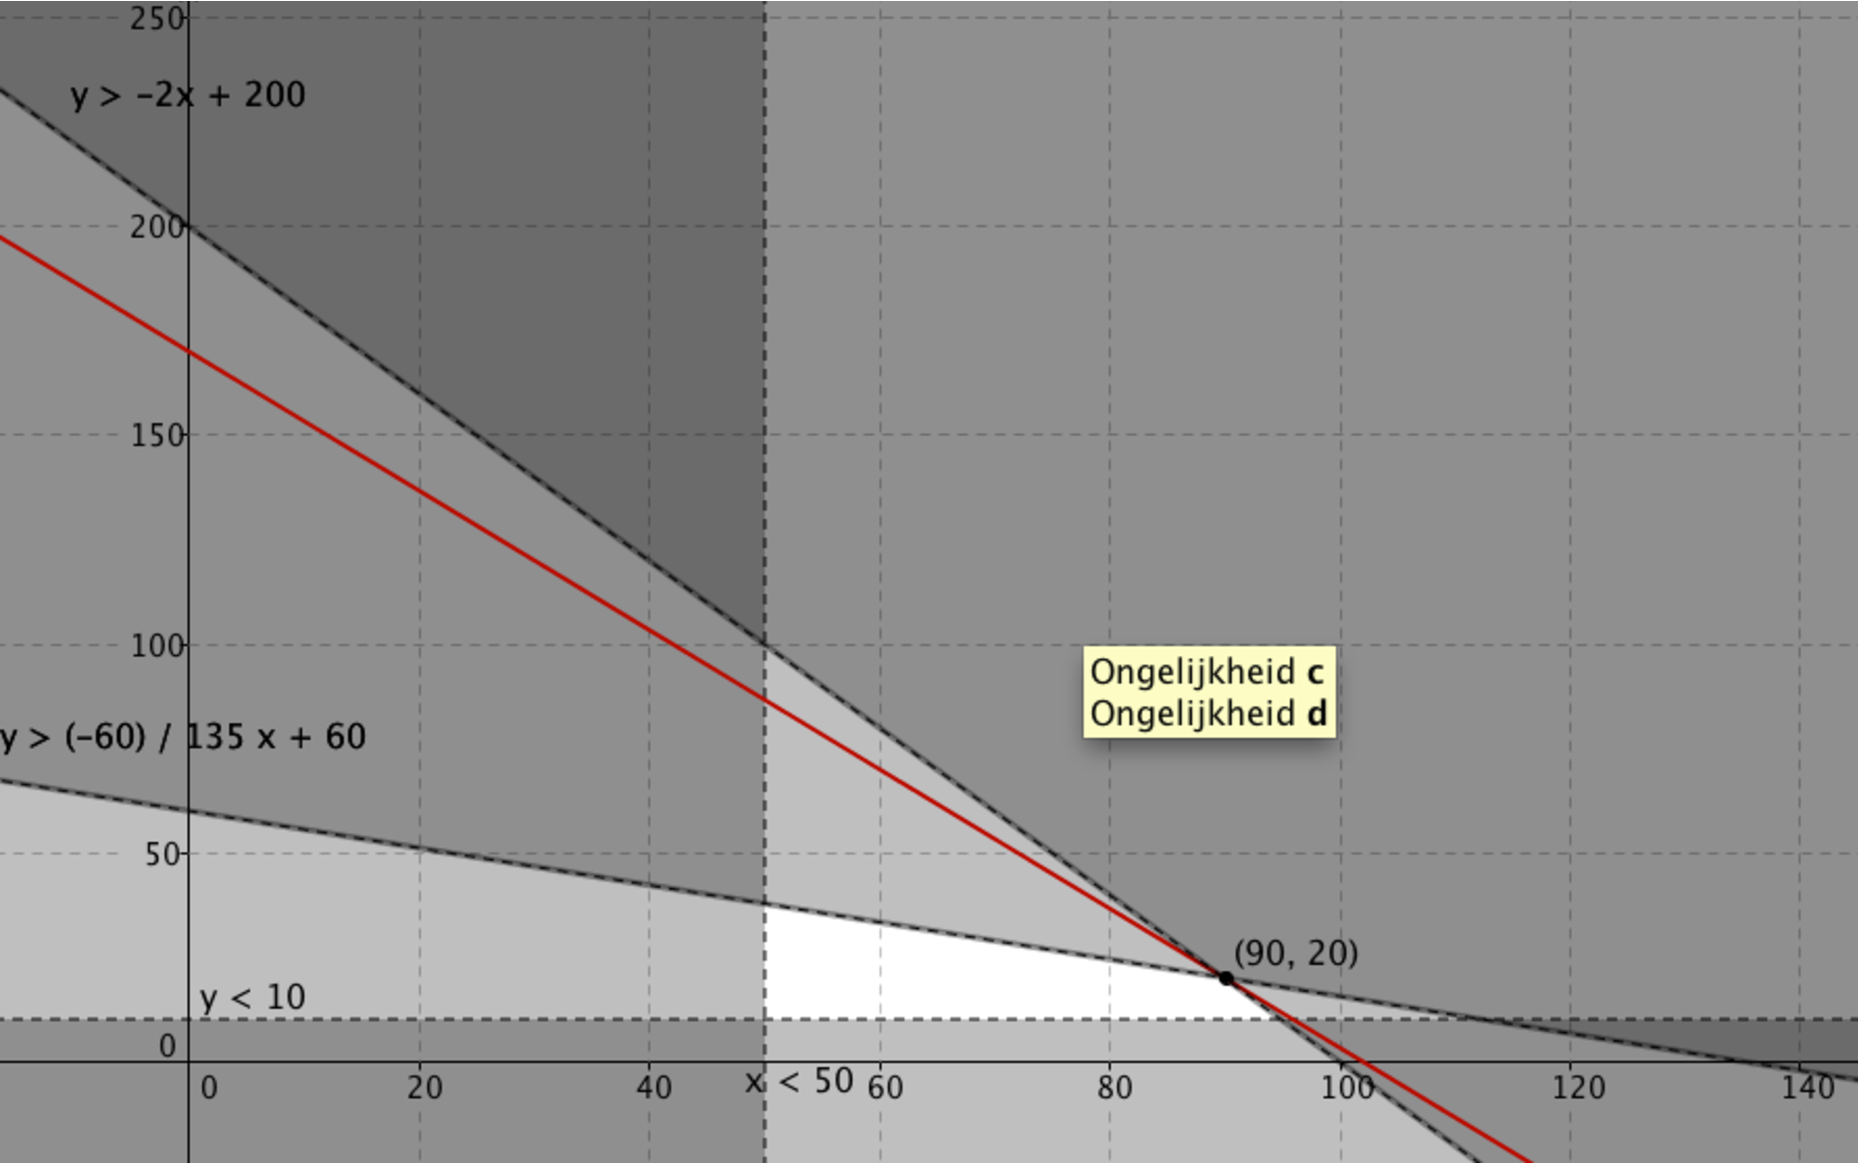
\includegraphics[width=0.8\textwidth]{oefeningen/FigurenLP/lofts}
\end{figure}
\end{Oplossing}
\begin{Oplossing}{5.1}
      \begin{itemize}
      \item $f$: lineair groeiproces met toename gelijk aan 7
      \item $g$: geen exponentiële en geen lineaire groei
      \item $h$: exponentieel groeiproces met groeifactor gelijk aan 1,1
      \item $k$: exponentieel groeiproces met groeifactor gelijk aan $\frac13$
      \item $m$: exponentieel groeiproces met groeifactor gelijk aan 5
      \item $w$: lineair groeiproces met toename gelijk aan $-2,6$
      \end{itemize}
      
\end{Oplossing}
\begin{Oplossing}{5.2}
     \begin{enumerate}
     \item $g_6=2$; $g_d=2^4=16$; $g_u=2^\frac{1}{6}=1,122462$
     \item (i) 12u; (ii) 12 uur geleden; (iii) tussen 18 en 24u
     \item $g_6(t)=100\cdot 2^t$; $g_d(t)=100\cdot 16^t$; $g_u(t)=100\cdot \left(2^\frac16 \right)^t$
     \end{enumerate}
     
\end{Oplossing}
\begin{Oplossing}{5.3}
      \begin{enumerate}
      \item $g_j=1,011$; $g_d=1,011^{10}$; $g_s=1,011^\frac{1}{2}$
      \item $M(t)=7\cdot 1,011^t$ in miljard aantal en $t$ het aantal jaren verstreken sinds 2011
      \item $M(39)=7\cdot 1,011^{39}=10,724896$
      \end{enumerate}
      
\end{Oplossing}
\begin{Oplossing}{5.4}
\begin{enumerate}
\item
$T_1(t)=10+\frac{t}{32}$ met $t$ het aantal meter grond dieper dan \SI{25}{\meter} onder de grond
\begin{enumerate}
\item Zoek $t$ zodat $T_1(t)=15$: op diepte van \SI{185}{\meter} onder de grond bedraagt de temperatuur \SI{15}{\celsius}.
\item $T_1(960)=40$, dus \SI{40}{\celsius}
\end{enumerate}
\item $T_2(t)=-5+\frac{t}{32}$ met $t$ het aantal meter onder de grond
\begin{enumerate}
\item Zoek $t$ zodat $T_2(t)=0$ geeft $t=160$, dus \SI{160}{meter} onder de grond bedraagt de temperatuur \SI{0}{\celsius}
\item $T_2(800)=20$, dus \SI{800}{meter} onder de grond is het \SI{20}{\celsius}
\end{enumerate}
\end{enumerate}
\end{Oplossing}
\begin{Oplossing}{5.5}
\begin{enumerate}
\item groeifactor per 1656 jaar: $\frac12$; groeifactor per jaar: $\left(\frac{1}{2}\right)^\frac{1}{1656}=0,9995815$ zodat de procentuele afname gelijk is aan \SI{0,0418480}{\percent}.
\item $R(t)=y_0\cdot \left(\frac{1}{2}^\frac{1}{1656}\right)^t$
\item $R(20)=\left(\frac{1}{2}^\frac{1}{1656}\right)^{20}=0,9916636$, dus er blijft \SI{0.9916636}{\gram} over.
\end{enumerate}
\end{Oplossing}
\begin{Oplossing}{5.6}
\begin{enumerate}
\item Na 2 jaar: \SI{67}{\percent}; na 3 jaar: \SI{55}{\percent}; na 6 jaar: \SI{30}{\percent}; na 10 jaar: \SI{14}{\percent}.
\item $12~500\cdot\frac{30}{100}=3800$
\end{enumerate}
\end{Oplossing}
\begin{Oplossing}{5.7}
  Groeifunctie: $B(t)=1,05^t$: bedrag in eurocent, $t$ jaar na 1830\\
  Nu is het 2012, dus bereken $B(182)=7185,42$\\
  In 2012 zou je \euros{71,85} ontvangen.
  
\end{Oplossing}
\begin{Oplossing}{6.2}
     Dikte van geplooide papier: $D(t)=2^t$.\\
     Zoek $t$ zodat $D(t)=20$. Dit geeft $t=\log20/\log 2=4,32$.\\
     Antwoord: na vijf keer plooien is dikte meer dan 2 cm.
     
\end{Oplossing}
\begin{Oplossing}{6.3}
      \begin{enumerate}
      \item $g_{10}=3$; $g_m=3^\frac{1}{10}$
      \item Waarde van aandeel in functie van de tijd: $B(t)=B(0)\cdot 3^\frac{t}{10}$ \\
      Zoek $t$ zodat $B(t)=5B(0)$. Dat geeft $t=\log5/\log3^\frac{1}{10}=14,65$, dus na 14,65 maanden.
      \end{enumerate}
      
\end{Oplossing}
\begin{Oplossing}{6.4}
      $J(t)=3355\cdot J_0\cdot \left( \frac12\right)^\frac{t}{8}$\\
      Zoek $t$ zodat $J(t)=J_0$\\
      $t=8\frac{\log \frac{1}{3355}}{\log\frac12}=93,70$, dus na 93,70 dagen.
      
\end{Oplossing}
\begin{Oplossing}{6.5}
    $C(t)=0,20\cdot C_0\cdot 0,9988^t$\\
    Zoek $t$ zodat $C(t)=C_0$\\
    $t=\frac{\log5}{\log0,9988}=-13411$, dus 13411 jaar geleden.
    
\end{Oplossing}
\begin{Oplossing}{6.6}
Groeifunctie van spaarboekje 1: $S_1(t)=1900\cdot 1,05^t$; \\Groeifunctie van spaarboekje 2: $S_2(t)=1000\cdot 2^\frac{t}{25}$\\
Zoek $t$ zodat $S_1(t)=2\cdot S_2(t)$, wat geeft $t=\frac{\log(19/20)}{\log(2^{1/25}/1,05)}=2,435$.\\
Antwoord: na 2,435 jaar is het bedrag van het spaarboekje dubbel zo groot als het bedrag op de rekening.
\end{Oplossing}
\begin{Oplossing}{6.7}
         De waarde van de Rembrandt: $R(t)=300000\cdot 1,20^{t/10}$\\
         De waarde van de Picasso: $P(t)=225000\cdot 1,05^t$\\
         Zoek $t$ zodat $P(t)=R(t)$, wat geeft $t=\log(300/225)/\log(1,05/1,20^{1/10})=9,41$.\\
         Antwoord: na 9,41 jaar zijn beide schilderijen evenveel waard.
      
\end{Oplossing}
\begin{Oplossing}{6.8}
	$A(t)=80\cdot 2^{t/20}$; $B(t)=100\cdot 1,023^t$;\\
	Zoek $t$ zodat $A(t)=B(t)$, wat geeft $t=\log(8/10)/\log(1,023/2^{1/20})=18,72$\\
	Antwoord: na 18,72 jaar zal het aantal inwoners gelijk zijn.
      
\end{Oplossing}
\begin{Oplossing}{6.9}
  		Groeifunctie die het gespaarde bedrag $t$ jaar na de zevende verjaardag weergeeft: $B(t)=400\cdot 1,07^t$\\
  		\begin{enumerate}
  		\item bedrag op rekening bij twaalfde verjaardag: $B(5)=561,02$
  		\item Zoek $t$ zodat $B(t)=800$, wat geeft $t=\log2/\log1,07=10,24$, dus als Wim 17,24 jaar is, heeft hij 800\euros op zijn rekening staan.
  		\end{enumerate}
      
\end{Oplossing}
\begin{Oplossing}{6.10}
Bedrag op rekening van kind 1: $B_1(t)=B_1\cdot 1,07^t$ met $t$ het aantal jaren sinds `nu'.\\
Bedrag op rekening van kind 2: $B_2(t)=B_2\cdot 1,07^t$ met $B_1+B_2=\num{10000}$; \\
Zoek $B_1$ en $B_2$ zodat $B_1(11)=B_2(6,5)$. Omdat $B_1+B_2=\num{10000}$, moeten we $B_1$ zoeken zodat
$B_1\cdot 1,07^{11}=(10000-B_1)\cdot 1,07^{6,5}$, wat geeft $B_1=4244$. \\
Antwoord: Nu wordt \euros{4244} en \euros{5755} belegd.\\
Op zijn  \'{e}\'{e}nentwintigste verjaardag zal het kind beschikken over \euros{8934}.
\end{Oplossing}
\begin{Oplossing}{6.11}
Eerst zoeken we de groeifactor uit de vergelijking:\\
$3000\cdot g^{8} = 4432,37$\\
Hieruit vinden we dat $g$ gelijk is aan $1,05$. Het kapitaal groeit dus met \SI{5}{\percent} per jaar.\\
Nu kunnen we berekenen wanneer het kapitaal aangegroeid is tot \euros{5000}\\
$3000\cdot 1,05^{t} = 5000$\\
$t = \log(5/3)/\log(1,05)$\\
$t = 10,46$\\
Hieruit vinden we dat het kapitaal $11$ jaar op de bank moet blijven staan vooraleer het is aangegroeid tot \euros{5000}.

   
\end{Oplossing}
\begin{Oplossing}{6.12}
$B(t)=\num{1124000}\cdot 0,9^{t/10}$ en $L(t)=\num{95500}\cdot 2^{t/8}$ met $t$ uitgedrukt in jaren. Na \SI{25,37} jaren telt Leuven evenveel inwoners als Brussel.
\end{Oplossing}
\begin{Oplossing}{7.1}
Je vindt enkele opgeloste oefeningen in tabellen~\ref{tab:logica1} tot en met \ref{tab:logica3}.
\begin{table}[htbp]\footnotesize
\centering
\caption{Oefening 7.1 - 1}
\begin{tabular}{cccccccc}
\toprule
$p$ & $q$ & $r$ & $q\en r$ & $p\of (q\en r)$ & $q\of r$ & $p\en (q\of r)$ & $(p\of (q\en r))\en \niet(p\en (q\of r))$ \\
\midrule
0 & 0 & 0 & 0 & 0 & 0 & 0 & 0 \\
0 & 0 & 1 & 0 & 0 & 1 & 0 & 0 \\
0 & 1 & 0 & 0 & 0 & 1 & 0 & 0 \\
0 & 1 & 1 & 1 & 1 & 1 & 0 & 1 \\
1 & 0 & 0 & 0 & 1 & 0 & 0 & 1 \\
1 & 0 & 1 & 0 & 1 & 1 & 1 & 0 \\
1 & 1 & 0 & 0 & 1 & 1 & 1 & 0 \\
1 & 1 & 1 & 1 & 1 & 1 & 1 & 0 \\
\bottomrule
\end{tabular}
\label{tab:logica1}
\end{table}

\begin{table}[htbp]\footnotesize
\centering
\caption{Oefening 7.1 - 2: contradictie}
\begin{tabular}{cccccc}
\toprule
$p$ & $q$ & $p\of q$ & $\niet(p\of q)$ & $p\en q$ & $\niet(p\of q)\en(p\en q)$ \\
\midrule
0 & 0 & 0 & 1 & 0 & 0 \\
0 & 1 & 1 & 0 & 0 & 0 \\
1 & 0 & 1 & 0 & 0 & 0 \\
1 & 1 & 1 & 0 & 1 & 0 \\
\bottomrule
\end{tabular}
\label{tab:logica2}
\end{table}

\begin{table}[htbp]\footnotesize
\centering
\caption{Oefening 7.1 - 3: tautologie}
\begin{tabular}{ccccc}
\toprule
$p$ & $q$ & $p\en \niet q$ & $\niet p \of q$ & $(p\en \niet q)\of (\niet p \of q)$ \\
\midrule
0 & 0 & 0 & 1 & 1 \\
0 & 1 & 0 & 1 & 1 \\
1 & 0 & 1 & 0 & 1 \\
1 & 1 & 0 & 1 & 1 \\
\bottomrule
\end{tabular}
\label{tab:logica3}
\end{table}
\end{Oplossing}
\begin{Oplossing}{7.8}
\begin{enumerate}
\item \verb+if (a<>3 & a<>4)| (b<=a)+
\item $p$: \texttt{a==3}; $q$: \texttt{a==4}; $r$: \texttt{b<=a}
\item $(\niet p \en \niet q)\of r$, of korter: $\niet(p \of q) \of r$
\item $(p\of q)\en \niet r$
\end{enumerate}
\end{Oplossing}
\begin{Oplossing}{7.9}
\begin{enumerate}
\item \verb/modulo(i+j,4)==0 & (modulo(i,2)<>0 & modulo (j,2)<>0)/
\item $p$: \verb/modulo(i+j,4)==0 /; $q$: \verb/modulo(i,2)==0 /; $r$: \verb/modulo (j,2)==0/
\item $p \en (\niet q \en \niet r)=p\en \niet (q \of r)$
\item $\niet p \of (q \of r)$
\end{enumerate}
\end{Oplossing}
\begin{Oplossing}{7.14}
\begin{enumerate}
\item
$a$: student heeft één punt verschil met linkerbuur\\
$b$: student heeft één punt verschil met rechterbuur\\
$c$: student heeft zelfde punt als linkerbuur\\
$d$: student heeft zelfde punt  als linkerbuur
\item \begin{enumerate}
\item $a \of b$
\item $\niet (a \of b)$
\item $c \of d$
\item $\niet (c \of d) $
\item $(a\of b)\of (c\of d)$
\item $(a\of b)\en \niet (c\of d)$
\item $\niet (a\of b)\en \niet (c\of d)$
\end{enumerate}
\end{enumerate}
\end{Oplossing}
\begin{Oplossing}{9.1}
\begin{enumerate}
\item  12.783185
\item - 42.875
\item 4
\item 1, -3
\item -3
\item 7555.9475
\end{enumerate}
   
\end{Oplossing}
\begin{Oplossing}{9.15}
Eén van de vele mogelijke oplossingen:
\begin{lstlisting}[caption={Een vector omkeren}, label=vectoromkeren]
function W=keerom(V)
  // schrijft vector V in omgekeerde volgorde
  W=V
  l=length(V)
  for i=1:l
    W(l+1-i)=V(i)
  end
endfunction
\end{lstlisting}
\end{Oplossing}
